\RequirePackage[l2tabu,orthodox]{nag}

% TODO: decide if one-sided/two-sided
%\documentclass[headsepline,footsepline,footinclude=false,fontsize=11pt,paper=a4,listof=totoc,bibliography=totoc,BCOR=12mm,DIV=12]{scrbook} % two-sided
\documentclass[headsepline,footsepline,footinclude=false,oneside,fontsize=11pt,paper=a4,listof=totoc,bibliography=totoc]{scrbook} % one-sided

% TODO: change citation style in settings
\PassOptionsToPackage{table,svgnames,dvipsnames}{xcolor}

\usepackage[utf8]{inputenc}
\usepackage[T1]{fontenc}
\usepackage[sc]{mathpazo}
\usepackage[ngerman,american]{babel}
\usepackage[autostyle]{csquotes}
% \usepackage[%
%   backend=biber,
%   url=false,
%   style=alphabetic,
%   maxnames=4,
%   minnames=3,
%   maxbibnames=99,
%   giveninits,
%   uniquename=init]{biblatex} % TODO: adapt citation style
\usepackage[natbib=true, 
            url=false, 
            style=authoryear,
            maxnames=2,
            date=year,
            ]{biblatex}
\addbibresource{bibliography.bib}

% \usepackage{natbib}
% \bibliographystyle{abbrvnat}
% \setcitestyle{authoryear} %Citation-related commands

\usepackage{graphicx}
\usepackage{scrhack} % necessary for listings package
\usepackage{listings}
\usepackage{lstautogobble}
\usepackage{tikz}
\usepackage{pgfplots}
\usepackage{pgfplotstable}
\usepackage{booktabs}
\usepackage[final]{microtype}
\usepackage{caption}
\usepackage[printonlyused]{acronym}
\AtBeginDocument{%
	\hypersetup{
		pdftitle=\getTitle,
		pdfauthor=\getAuthor,
	}
}
\usepackage{ifthen}
\usepackage{amsmath}
\usepackage{amssymb}
\usepackage{amsthm}
\usepackage{amsfonts}

\usepackage{xcolor}
\definecolor{standardblue}{rgb}{0.149,0.580,0.871}
\usepackage[colorlinks,citecolor=standardblue]{hyperref}


% for fachschaft_print.pdf
\makeatletter
\if@twoside
	\typeout{TUM-Dev LaTeX-Thesis-Template: twoside}
\else
	\typeout{TUM-Dev LaTeX-Thesis-Template: oneside}
\fi
\makeatother

\addto\extrasamerican{
	\def\lstnumberautorefname{Line}
	\def\chapterautorefname{Chapter}
	\def\sectionautorefname{Section}
	\def\subsectionautorefname{Subsection}
	\def\subsubsectionautorefname{Subsubsection}
}

\addto\extrasngerman{
	\def\lstnumberautorefname{Zeile}
}

% Themes
\ifthenelse{\equal{\detokenize{dark}}{\jobname}}{%
  % Dark theme
  \newcommand{\bg}{black} % background
  \newcommand{\fg}{white} % foreground
  \usepackage[pagecolor=\bg]{pagecolor}
  \color{\fg}
}{%
  % Light theme
  \newcommand{\bg}{white} % background
  \newcommand{\fg}{black} % foreground
}

% \bibliography{bibliography}

\setkomafont{disposition}{\normalfont\bfseries} % use serif font for headings
\linespread{1.05} % adjust line spread for mathpazo font

% Add table of contents to PDF bookmarks
\BeforeTOCHead[toc]{{\cleardoublepage\pdfbookmark[0]{\contentsname}{toc}}}

% Define TUM corporate design colors
% Taken from http://portal.mytum.de/corporatedesign/index_print/vorlagen/index_farben
\definecolor{TUMBlue}{HTML}{0065BD}
\definecolor{TUMSecondaryBlue}{HTML}{005293}
\definecolor{TUMSecondaryBlue2}{HTML}{003359}
\definecolor{TUMBlack}{HTML}{000000}
\definecolor{TUMWhite}{HTML}{FFFFFF}
\definecolor{TUMDarkGray}{HTML}{333333}
\definecolor{TUMGray}{HTML}{808080}
\definecolor{TUMLightGray}{HTML}{CCCCC6}
\definecolor{TUMAccentGray}{HTML}{DAD7CB}
\definecolor{TUMAccentOrange}{HTML}{E37222}
\definecolor{TUMAccentGreen}{HTML}{A2AD00}
\definecolor{TUMAccentLightBlue}{HTML}{98C6EA}
\definecolor{TUMAccentBlue}{HTML}{64A0C8}

% Settings for pgfplots
\pgfplotsset{compat=newest}
\pgfplotsset{
  % For available color names, see http://www.latextemplates.com/svgnames-colors
  cycle list={TUMBlue\\TUMAccentOrange\\TUMAccentGreen\\TUMSecondaryBlue2\\TUMDarkGray\\},
}

% Settings for lstlistings
\lstset{%
  basicstyle=\ttfamily,
  columns=fullflexible,
  autogobble,
  keywordstyle=\bfseries\color{TUMBlue},
  stringstyle=\color{TUMAccentGreen},
  captionpos=b
}

\newcommand{\R}{\mathbb{R}}
\newcommand{\calD}{\mathcal{D}}
\newcommand{\calL}{\mathcal{L}}
\newcommand{\bbE}{\mathbb{E}}
\newcommand{\z}{\mathbb{z}}
\newcommand{\U}{\mathcal{U}}
\newcommand{\N}{\mathcal{N}}
\newcommand{\divergence}{\operatorname{div}}
\newcommand{\trace}{\operatorname{Tr}}
\newcommand{\Cov}{\operatorname{Cov}}

\newcommand{\Lfm}{\mathcal{L}_{\text{FM}}(\theta)}
\newcommand{\Lcfm}{\mathcal{L}_{\text{CFM}}(\theta)}


% TODO: change thesis information
\newcommand*{\getUniversity}{Technische Universität München}
\newcommand*{\getFaculty}{Informatics}
\newcommand*{\getDegree}{Informatics}
\newcommand*{\getSchool}{Computation, Information and Technology}
\newcommand*{\getTitle}{Thesis title}
\newcommand*{\getTitleGer}{Titel der Abschlussarbeit}
\newcommand*{\getAuthor}{Author}
\newcommand*{\getDoctype}{Master's Thesis}
\newcommand*{\getSupervisor}{Supervisor}
\newcommand*{\getAdvisor}{Advisor}
\newcommand*{\getSubmissionDate}{Submission date}
\newcommand*{\getSubmissionLocation}{Munich}

\begin{document}

% Set page numbering to avoid "destination with the same identifier has been already used" warning for cover page.
% (see https://en.wikibooks.org/wiki/LaTeX/Hyperlinks#Problems_with_Links_and_Pages).
\pagenumbering{alph}
\begin{titlepage}
  % HACK for two-sided documents: ignore binding correction for cover page.
  % Adapted from Markus Kohm's KOMA-Script titlepage=firstiscover handling.
  % See http://mirrors.ctan.org/macros/latex/contrib/koma-script/scrkernel-title.dtx,
  % \maketitle macro.
  \oddsidemargin=\evensidemargin\relax
  \textwidth=\dimexpr\paperwidth-2\evensidemargin-2in\relax
  \hsize=\textwidth\relax

  \centering

  \IfFileExists{logos/tum-\fg.pdf}{%
    \includegraphics[height=20mm]{logos/tum-\fg.pdf}
  }{%
    \vspace*{20mm}
  }

  \vspace{5mm}
  {\huge\MakeUppercase{School of \getSchool{} --- \getFaculty{}} \par}

  \vspace{5mm}
  {\large\MakeUppercase{\getUniversity{}} \par}

  \vspace{15mm}
  {\Large \getDoctype{} in \getDegree{} \par}

  \vspace{10mm}
  {\huge\bfseries \getTitle{} \par}

  \vspace{10mm}
  {\LARGE \getAuthor{}}

  \IfFileExists{logos/faculty-\fg.pdf}{%
    \vfill{}
    \includegraphics[height=20mm]{logos/faculty-\fg.pdf}
  }{}
\end{titlepage}


\frontmatter{}

\begin{titlepage}
  \centering

  \IfFileExists{logos/tum-\fg.pdf}{%
    \includegraphics[height=20mm]{logos/tum-\fg_alt.pdf}
  }{%
    \vspace*{20mm}
  }

  \vspace{5mm}
  {\huge\MakeUppercase{School of \getSchool{} --- \getFaculty{}} \par}

  \vspace{5mm}
  {\large\MakeUppercase{\getUniversity{}} \par}

  \vspace{20mm}
  {\Large \getDoctype{} in \getDegree{} \par}

  \vspace{15mm}
  {\huge\bfseries \getTitle{} \par}

  \vspace{10mm}
  {\huge\bfseries \foreignlanguage{ngerman}{\getTitleGer{}} \par}

  \vspace{15mm}
  \begin{tabular}{l l}
    Author:          & \getAuthor{}         \\
    Examiner:      & \getSupervisor{}     \\
    Supervisor:         & \getAdvisor{}        \\
    Submission Date: & \getSubmissionDate{} \\
  \end{tabular}
\end{titlepage}

\thispagestyle{empty}
\vspace*{0.8\textheight}
\noindent
I confirm that this \MakeLowercase{\getDoctype{}} is my own work and I have documented all sources and material used.

\vspace{15mm}
\noindent
\getSubmissionLocation{}, \getSubmissionDate{} \hspace{\fill} \getAuthor{}

\cleardoublepage{}

% \addcontentsline{toc}{chapter}{Acknowledgments}
\thispagestyle{empty}

\vspace*{20mm}

\begin{center}
    {\usekomafont{sectioning}\usekomafont{section} Acknowledgments}
\end{center}

\vspace{10mm}

%TODO: Acknowledgments

\cleardoublepage{}

\chapter{\abstractname}

Deep generative models such as flow and diffusion models have proven to be effective in modeling high-dimensional and complex data types such as videos or proteins, and this has motivated their use in different data modalities, such as neural network weights. A generative model of neural network weights would be useful for a diverse set of applications, such as Bayesian deep learning, learned optimization, and transfer learning. However, the existing work on weight-space generative models often ignores the symmetries of neural network weights, or only takes into account a subset of them. Modeling those symmetries, such as permutation symmetries between subsequent layers in an MLP, the filters in a convolutional network, or scaling symmetries arising with the use of non-linear activations, holds the potential to make weight-space generative modeling more effcient by effectively reducing the dimensionality of the problem. 

In this light, we aim to design generative models in weight-space that more comprehensively respect the symmetries of neural network weights. We build on recent work on generative modeling with flow matching, and weight-space graph neural networks to design three different weight-space flows. Each of our flows takes a different approach to modeling the geometry of neural network weights, and thus allows us to explore the design space of weight-space flows in a principled way. Our results confirm that modeling the geometry of neural networks more faithfully leads to more effective flow models that can generalize to different tasks and architectures, and we show that while our flows obtain competitive performance with orders of magnitude fewer parameters than previous work, they can be further improved by scaling them up. We conclude by listing potential directions for future work on weight-space generative models.
\microtypesetup{protrusion=false}
\tableofcontents{}
\microtypesetup{protrusion=true}

\mainmatter{}

% Background
% •⁠  ⁠bayesian dl
% •⁠  ⁠⁠diffusion/fm
% •⁠  ⁠⁠geometry of loss landscapes
% •⁠  ⁠⁠graph neural net and metanets
% Method/ design choices
% •⁠  ⁠fm design choices
% Results
% Discussion
% Future work

\begin{table}[t!]
    \centering
    \begin{tabular}{cl}
        \toprule
        \textbf{Notation} & \textbf{Explanation} \\
        \midrule

        $\theta$             & Parameters of a neural network \\
        $(x,y) \in \calD$    & Dataset with inputs $x$ and labels/targets $y$ \\
        $v_t$                & Time-dependent vector field  \\
        $\phi_t$             & Flow map from time 0 to time $t$ \\
        
        

        \bottomrule
    \end{tabular}
    \caption{\label{tab:notation} Summary of notation used throughout the thesis.}
\end{table}
\clearpage

% !TeX root = ../main.tex
% Add the above to each chapter to make compiling the PDF easier in some editors.

\begin{figure}[t!]
    \centering
    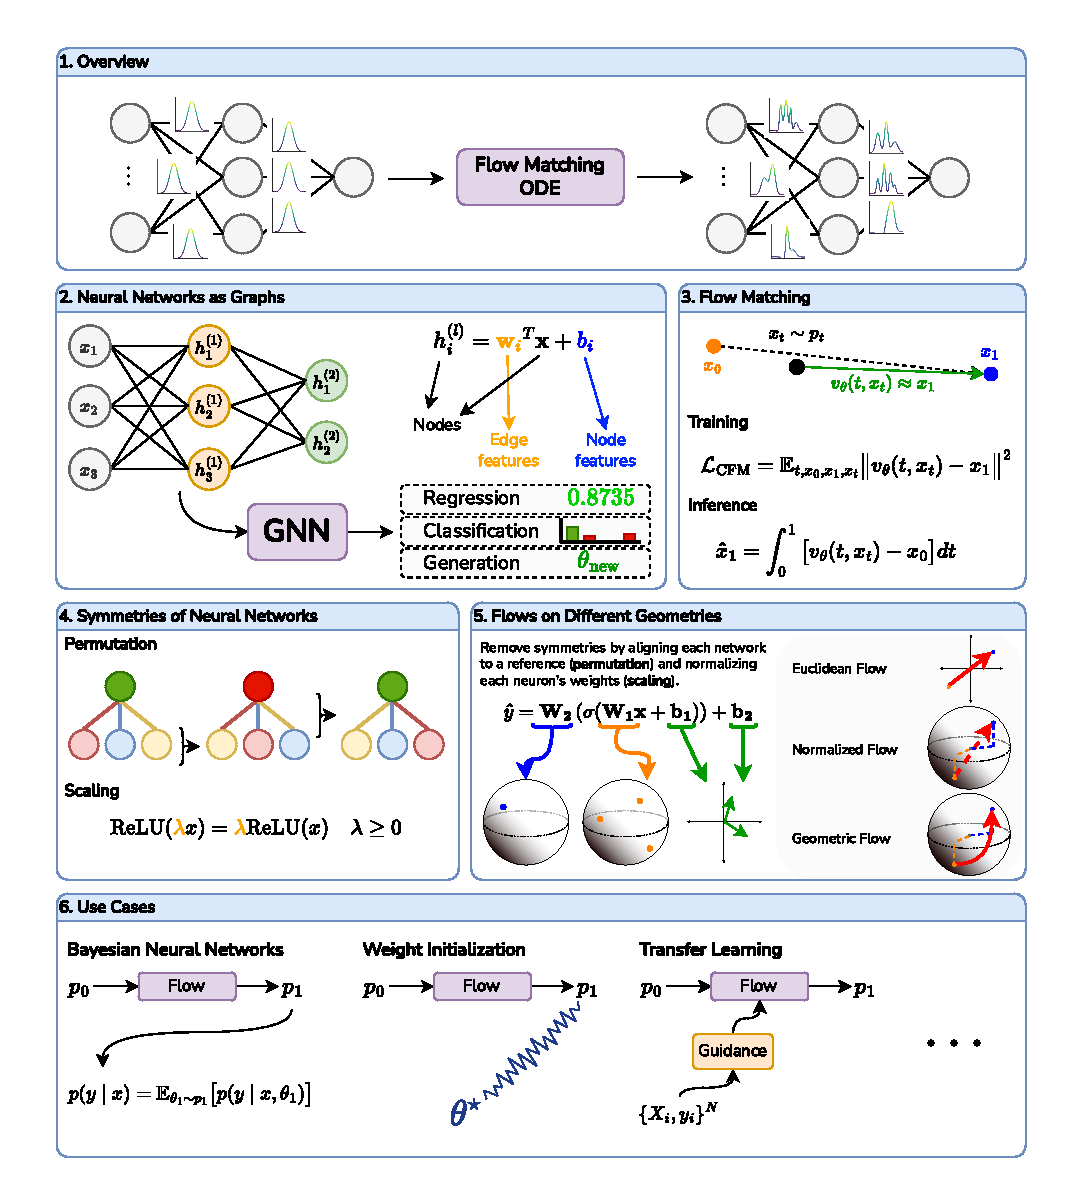
\includegraphics[width=\linewidth]{figures/weightflow.drawio.pdf}
    \caption{\label{fig:main}\textbf{Overview of our weight-space flow.} We aim to learn a flow in weight-space \textit{(1)}, processing neural networks with GNNs \textit{(2)}, using flow matching \textit{(3)} and taking into account the symmetries of neural network weights \textit{(4)}. We propose three different flows \textit{(5)} and potential use cases include Bayesian neural networks, learned weight initialization, or transfer learning \textit{(6)}.}
\end{figure}

\chapter{Introduction}\label{chapter:introduction}

Deep generative models such as diffusion and flow models that have led to significant developments in image generation \citep{esserScalingRectifiedFlow2024b} or biological applications such as protein structure prediction \citep{abramsonAccurateStructurePrediction2024} have also been applied to neural network weights \citep{peeblesLearningLearnGenerative2022,schurholtHyperRepresentationsLearningPopulations2024a}. However, the existing works do not take into account the geometry of neural networks arising from permutation and scaling symmetries, or only consider the permutation symmetries. We attempt to fill this gap by building flow models that learn a vector field to transport a prior over neural network to the posterior for a specific task through the flow matching framework \citep{lipmanFlowMatchingGuide2024}, processing neural network weights with permutation-invariant graph neural networks \citep{kofinasGraphNeuralNetworks2024,limGraphMetanetworksProcessing2023} and propose three candidate designs differing on how they handle the underlying geometry. Figure \ref{fig:main} gives an overview of our approach, and we summarize the main points in this Introduction. 

\subsubsection{Symmetries of Neural Networks (Chapter \ref{section:geometry_of_nns})}

Neural networks are subject to various symmetries, i.e. transformations of the network parameters that leave the function it is computing unchanged, and this topic has been an active research topic since the early days of neural network research \citep{hecht-nielsenALGEBRAICSTRUCTUREFEEDFORWARD1990}. For example in an MLP, permuting the neurons in one layer together with the outgoing weights preserves the function, as does similarly permuting the channels in a convolutional neural network. Non-linear activation functions induce further scaling symmetries \citep{godfreySymmetriesDeepLearning2022}; e.g. for a constant $\lambda \geq 0$, $\text{ReLU}(\lambda x) = \lambda \text{ReLU}(x)$, which means scaling the input weights to a neuron and applying the inverse scaling to the outgoing weights again preserves neural network's function. In addition to these static symmetries, other forms of symmetries might arise from the structure of the data, or dynamically during phases of training \citep{zhaoFindingSymmetryNeural2024}. 

Accounting for these symmetries in a weight-space learning task by using architectures with the correct inductive biases, through data augmentation \citep{shamsianImprovedGeneralizationWeight2024} or by removing the symmetries by mapping neural networks to canonical representations \citep{pittorinoDeepNetworksToroids2022} as we will do can reduce the effective dimensionality of the problem and make weight-space learning more scalable. 

\subsubsection{Neural Networks as Graphs (Chapter \ref{section:wsl})}

A neural network can naturally be modeled as a graph, and this has fueled a recent line of work building graph neural networks (GNNs) that take as input other neural networks \citep{kofinasGraphNeuralNetworks2024,limGraphMetanetworksProcessing2023,kalogeropoulosScaleEquivariantGraph2024}. The nodes often correspond to the neurons in an MLP or channels in a convolutional network and the edges to the weights. Used with the appropriate positional encodings, this graph formalism provides an effective way of handling the permutation symmetries of various kinds of neural networks including transformers and neural networks with residual connections, and has also been extended to account for scaling symmetries \citep{kalogeropoulosScaleEquivariantGraph2024}. Furthermore, since a GNN is not restricted to graphs with a certain structure, weight-space GNNs have the additional benefit that the same GNN can be used to process different neural networks, even those with different architectures altogether.

In building our flows, we also process neural networks using GNNs, more specifically the Relational Transformer model \citep{diaoRelationalAttentionGeneralizing2023,kofinasGraphNeuralNetworks2024} that incorporates an attention mechanism with edge updates. 

\subsubsection{Generative Modeling with Flow Matching (Chapter \ref{section:flow_models})}

Flow matching (FM) \citep{lipmanFlowMatchingGenerative2023,albergoStochasticInterpolantsUnifying2023,liuFlowStraightFast2022,tongImprovingGeneralizingFlowbased2023} generalizes diffusion models with a more flexible framework and a simple simulation-free regression objective. Given two sampleable marginal distributions $p_0$ and $p_1$, a coupling $(x_0, x_1)$ is sampled from a joint distribution, and $x_t$ from the conditional intermediate distribution $p_t(x_t \mid x_0, x_1)$ with $t$ sampled within the interval $[0,1]$. A neural network (velocity model) is then trained to predict the conditional velocity $u_t(x_t \mid x_0, x_1)$, such as $x_1 - x_0$. Marginalizing over the joint coupling then results in a time-dependent vector field that transforms $p_0$ to $p_1$, which is estimated by solving a differential equation with the velocity given by the trained velocity model. This flow matching framework can also be extended to data with more general geometries such as Riemannian manifolds \citep{chenRiemannianFlowMatching2023}. 

We will train our models using flow matching, with a Gaussian prior and the posterior samples collected through the neural networks' optimization trajectories, experimenting with different couplings. Our slightly modified flow matching training setup is described in more detail in Section \ref{sec:fm_training}.

\subsubsection{Flows with Different Geometries (Chapter \ref{chapter:method})}

We consider ReLU MLPs, and to remove the permutation symmetries, we align all neural networks to the same reference network using the rebasin operation \citep{ainsworthGitReBasinMerging2023,penaReBasinImplicitSinkhorn2023} that permutes a network's weights to minimize the loss barrier between two networks. To handle the scaling symmetries, we build on the canonicalization procedure of \citep{pittorinoDeepNetworksToroids2022}, where each neuron's incoming weights are normalized and its outgoing weights are inversely scaled to preserve the function being computed; the last layer is further normalized globally in classification networks. This gives the neural network a product geometry, with the bias vectors as Euclidean vectors, intermediate neurons on the hypersphere, and the last layer (optionally) on the hypersphere as a whole. 

We then compare three different kinds of flows: first a Euclidean flow that ignores the scaling symmetries, then a Normalized flow with the weights embedded in the product geometry but with the velocity field defined in Euclidean space (i.e. inside the hyperspheres), and finally a Geometric flow with the velocity field defined on the product geometry as well using the Riemannian Flow Matching framework \citep{chenRiemannianFlowMatching2023}. 

\subsubsection{Overview of Results (Chapter \ref{chapter:results})}

We evaluate our flows on a variety of tasks after training them on samples obtained with gradient-based optimization methods and show that for small networks on relatively easier tasks, they can directly generate weights matching or sometimes exceeding the performance of optimized weights. On more complex tasks and larger models, while direct generation does not match the quality of optimized weights, Bayesian model averaging over a number of samples leads to comparable predictive performance. Then we show that a flow trained on weights from one task can be transferred to another task, either by using the sampled weigths as learned initializations, or by guiding the sampling process with task gradients. Finally we show that in particular the Euclidean and Geometric flows can also generalize to different architectures for the same base task, and that there are still gains to be made by further scaling up our models. 

\section{Reproducibility and Guide to Code}




% !TeX root = ../main.tex
% Add the above to each chapter to make compiling the PDF easier in some editors.

% \chapter{Background \& Related Work}\label{chapter:Background}

% !TeX root = ../main.tex
% Add the above to each chapter to make compiling the PDF easier in some editors.

\chapter{Bayesian Deep Learning}\label{section:bayesian_dl}

A primary use case for a generative model over neural network weights is in Bayesian deep learning, where it can allow efficient inference by transporting the prior distribution to the posterior. Thus, to motivate the rest of the discussion, we first give an overview of concepts from Bayesian deep learning. Section \ref{section:bayesian_concepts} is a general introduction, followed by a review of inference methods (Laplace approximations, variational inference, MCMC-based methods) typically used for Bayesian neural networks.

\section{General Concepts} \label{section:bayesian_concepts}

Bayesian deep learning aims to quantify the uncertainty in neural networks through probability distributions over their parameters, rather than obtaining a single solution by an SGD-like optimization method (refer to \citep{mackayBayesianMethodsAdaptive1992, nealBayesianLearningNeural1996} for foundational work and \citep{goanBayesianNeuralNetworks2020,arbelPrimerBayesianNeural2023} for more recent reviews). With the \textit{posterior} distribution $p(\theta \vert \calD)$ over weights $\theta$ conditioned on the dataset $\calD$, predictions are obtained via \textit{Bayesian model averaging}:
\begin{equation} \label{eq:model_averaging}
    p(y \vert x, \calD) 
    = \bbE_{\theta \sim p(\theta \vert \calD)} \left[ p(y\vert x, \theta) \right]
    = \int p(y \vert x, \theta) p(\theta \vert \calD) d\theta,
\end{equation}
where the prediction is an expectation over the posterior. Note that since the forward pass through the model $p(y \vert x, \theta)$, is deterministic, the uncertainty in predictions results solely from the uncertainty over parameters. To bring things together, Bayesian inference over neural network weights consists of three steps:
\begin{enumerate}
    \item Specify prior $p(\theta)$.
    \item Compute/sample posterior $p(\theta \vert \calD) \propto p(\calD \vert \theta) p(\theta)$.
    \item Average predictions over the posterior. 
\end{enumerate}
The last step only requires forward passes through the model and thus is straightforward. The first two steps require deeper consideration. 

\section{Priors}

Specifiying a prior mainly consists of two choices: specifying an architecture, and specifying a probability distribution over the weights. A standard choice for a prior distribution is an isotropic Gaussian, which is an uninformative prior but therefore widely applicable and flexible. 

Different architectural decisions also induce different distributions over functions, even if the flattened weight vectors are identical, meaning that the choice of an architecture further specifies a prior in function space. As a simple example, keeping the depth and width of a neural network constant, even just changing the activation function from a ReLU to a sigmoid results in a different distribution of functions. The functional distribution can also be specified in a more deliberate way; e.g. a translation-invariant convolutional neural network, or a group-equivariant network \citep{cohenGroupEquivariantConvolutional2016} puts probability mass only on functions satisfying certain equivariance constraints depending on the task at hand. 

We keep this discussion short since the choice of a prior has tangential impact in the rest of the presentation, and we refer to recent reviews such as \citep{fortuinPriorsBayesianDeep2022} for a more detailed treatment of Bayesian neural network priors. 

\section{Inference} \label{section:bayesian_inference}

Inference in BNNs is a rich research area covering a wide range of methods. In this section we give an overview of key methods used to approximate BNN posteriors, and refer to works such as \citep{arbelPrimerBayesianNeural2023} and \citep{murphyProbabilisticMachineLearning2023} for more comprehensive treatments. 

\subsection{Laplace Approximation}

A Laplace approximation to the posterior \citep{mackayPracticalBayesianFramework1992} is essentially a Gaussian distribution centered at the MAP estimate of the posterior, with the covariance matrix given by the log likelihood's Hessian's inverse. This intuitiveyl corresponds to a local second-order Taylor expansion around the MAP estimate. 

A Laplace approximation is simple and fast, but ignores the posterior's multi-modality as it only captures a single mode. Nevertheless, it has been an active topic of research \citep{daxbergerLaplaceReduxEffortless2021} due to its simplicity and for use cases benefiting from local posterior estimates. 

\subsection{Variational Inference}

In a variational approximation, the posterior is estimated with a parametric distribution whose parameters are learned to minimize the KL-divergence between the posterior and the variational approximation; e.g. learning the mean and covariance matrix of a Gaussian distribution. The parameters are often learned to optimize the evidence lower bound (ELBO) using reparametrization tricks \citep{kingmaAutoEncodingVariationalBayes2022b,blundellWeightUncertaintyNeural2015a}. 

Variational approximatinos trade off expressivity for tractable optimization and thus can learn more complex distributions than a Gaussian, e.g. by accounting for symmetries in a neural network's posterior landscape \citep{gelbergVariationalInferenceFailures2024}. Nevertheless, KL-based objectives may require a large number of likelihood evaluations and often suffer from mode collapse, where the approximation captures only one mode of the distribution \citep{felardosDesigningLossesDatafree2023}. 

\subsection{Sampling-Based Inference}

Rather than parametrize or approximate the posterior distribution, sampling-based methods which our flow is a part of, attempt to sample from the posterior directly. Two main approaches to sampling are Monte Carlo methods \citep{barbuMonteCarloMethods2020} such as Markov chain Monte Carlo or importance sampling, and map-based methods \citep{marzoukSamplingMeasureTransport2016} such as normalizing flows \citep{rezendeVariationalInferenceNormalizing2015}.

\subsubsection{Monte Carlo Methods}

Monte carlo methods are designed around a few core ideas such that the samples are asymptotically from the true posterior, and are often used to compute expectations of the form
\begin{equation} \label{eq:expectation}
    \bbE_{x \sim p(x)} \left[ h(x) \right].
\end{equation}
A simple approach is Importance Sampling (IS) \citep{kahnMethodsReducingSample1953}, where samples from a proposal distribution $q$ are reweighted with $w(x) = p(x)/q(x)$ to estimate the expectation in Equation \ref{eq:expectation}:
\begin{equation}
    \bbE_{x \sim q(x)} \left[ \frac{p(x)}{q(x)} h(x) \right]
    = \int q(x) \frac{p(x)}{q(x)} h(x) dx = \int p(x)h(x) dx = \bbE_{x \sim p(x)} \left[ h(x) \right].
\end{equation}
While IS does not require sampling from the posterior, the rate of convergence for the estimate depends on the variance of the IS weights, i.e. how well the proposal distribution aligns with the true posterior. 

Alternatively, Markov chain Monte Carlo (MCMC) methods such Hamiltonian Monte Carlo \citep{nealMCMCUsingHamiltonian2011}, Stochastic Gradient Monte Carlo \citep{maCompleteRecipeStochastic2015}, or Langevin Monte Carlo \citep{robertsExponentialConvergenceLangevin1996} construct a Markov chain of samples that eventually converges (mixes) to the true posterior. This is often achieved through a Metropolis-Hastings correction step \citep{metropolisEquationStateCalculations1953,hastingsMonteCarloSampling1970} where a proposed step $z$ from the current state $x$ is accepted with probability 
\begin{equation}
    a(x,z) = \min \left\{ 1, \frac{p(z)}{p(x)} \frac{q(z,x)}{q(x,z)} \right\}
\end{equation}
where $q(x, z)$ gives the transition probability from $x$ to $z$. 

While chain-based methods are heavily used in practice, they suffer from various shortcomings such as generating correlated rather than independent samples, and requiring a large number of likelihood evaluations some of which is later rejected. Measuring the convergence of a chain is also challenging, lacking concrete rules. 

\subsubsection{Map-Based Sampling}

Map-based methods \citep{marzoukSamplingMeasureTransport2016} are instead use a map $T:\R^n \to \R^n$ that transforms samples from the prior distribution $q$ to samples from the posterior $p$, such that the push-forward of the prior gives the posterior distribution: $T_\sharp  q = p$. Such a map can generate independent, uncorrelated samples without any likelihood evaluations which is a desirable property. 

The theory of map-based sampling is closely related to optimal transport (OT) \citep{peyreComputationalOptimalTransport2020,santambrogioOptimalTransportApplied2015} with a history going back to the 18th century \citep{mongeMemoireTheorieDeblais1781}, where the goal is to find the map $T$ that minimizes some cost $c(x, T(x))$ such as Euclidean distance. Under the later relaxation of the problem by Kantorovich \citep{kantorovitchTranslocationMasses1958} to joint distributions rather than deterministic maps to minimize the cost over the joint distribution with marginal constraints, the optimal map is guaranteed to exists given mild conditions. 
 
Nevertheless, while a map-based approach has benefits over an MCMC method such as providing less ambigous convergence criteria by reducing the problem to optimization, the optimal map is often hard to find, and therefore approximate maps are used instead. Such maps can be learned as static \citep{rezendeVariationalInferenceNormalizing2015} or continuous normalizing flows \citep{chenNeuralOrdinaryDifferential2018a} which have seen risign interest recently with developments such as flow matching which we now turn to. 



% !TeX root = ../main.tex
% Add the above to ea  ch chapter to make compiling the PDF easier in some editors.

\chapter{Flow Models}\label{section:flow_models}

\section{Overview}

We train our flow using \textit{flow matching} \citep{lipmanFlowMatchingGenerative2023,albergoStochasticInterpolantsUnifying2023,liuFlowStraightFast2022}, which generalizes diffusion models with a more flexible design space. In this section we first formulate the flow matching objective (Sec. \ref{section:flow_matching}), explain the design choices it enables (Sec. \ref{section:design_choices}), and describe in more detail how likelihoods (Sec. \ref{section:computing_likelihoods}) can be computed using a flow model. 

\section{Flow Matching} \label{section:flow_matching}

Flow matching, first proposed in \citep{lipmanFlowMatchingGenerative2023,albergoStochasticInterpolantsUnifying2023,liuFlowStraightFast2022} (see \citep{lipmanFlowMatchingGuide2024} for a recent comprehensive overview), aims to solve the problem of \textit{dynamic transport}, i.e. finding a time-dependent vector field to transport the source (prior) distribution $p_0$ to the target (data) distribution $p_1$. More formally, the vector field $u_t: [0,1] \times \R^d \to \R^d$ leads to the ordinary differential equation (ODE)
\begin{equation} \label{eq:ode}
    dx = u_t(x) dt
\end{equation}
and induces a \textit{flow} $\phi: [0,1] \times \R^d \to \R^d$ that gives the solution to the ODE at time $t$ with starting point $x_0$, such that 
\begin{align}
    \frac{d}{dt} \phi_t(x_0) &= u_t(\phi_t(x_0)) \\
    \phi_0(x_0) &= x_0.
\end{align}
Starting with $p_0$, transformed distributions $p_t$ can then be defined using this flow with the push-forward operation
\begin{equation}
    p_t := [\phi_t]_\# (p_0)
\end{equation} 
and the instantaneous change in the density satisfies the \textit{continuity equation}
\begin{equation}
    \frac{\partial p}{\partial t} = - \nabla \cdot (p_t u_t)
\end{equation}
which means that probability mass is conserved during the transformation. With these formulations, we say the vector field $u_t$ \textit{generates} the \textit{probability path} (also called \textit{interpolant}) $p_t$.

\subsection{The Objective}

The formulation above could also be applied to traditional continuous normalizing flows (CNFs) \citep{chenNeuralOrdinaryDifferential2018a}, and flow matching is an instantiation of CNFs. However, continuous normalizing flows have in the past been trained using objectives which required solving and then backpropagating through the ODE, such as KL-divergence or other likelihood-based objectives, which made training costly. This problem was later addressed with diffusion models and their simpler regression objectives such as score matching and denoising \citep{sohl-dicksteinDeepUnsupervisedLearning2015, songScoreBasedGenerativeModeling2021a,hoDenoisingDiffusionProbabilistic2020} that proved to be very effective. The flow matching objective is also formulated as a simulation-free regression objective, and is more flexible than the diffusion objectives. 

As explained in Section \ref{section:flow_matching}, the goal in flow matching is to learn a vector field $v_\theta: [0,1] \times \R^d \to \R^d$ parametrized by a neural network.\footnote{For conciseness, we interchangeably use the subscripts for vector fields to denote time ($u_t(x)$) and parameters ($v_\theta(t,x)$).} If we know the ground truth vector field $u$ and can sample from the intermediate $p_t$'s, we can directly optimize the flow matching objective 
\begin{equation} \label{eq:fm_objective}
    \Lfm := \bbE_{t \sim \U(0,1), x_t \sim p_t(x)} \Vert v_\theta(t, x_t) - u_t(x_t) \Vert ^2
\end{equation}
by first sampling a time point $t$ and then $x_t \sim p_t$. However in practice, we neither have a closed form expression for $u$ nor can sample from an arbitrary $p_t$ without integrating the flow. 

The \textit{conditional flow matching} (CFM) framework first introduced in \citep{lipmanFlowMatchingGenerative2023} and then extended in \citep{tongImprovingGeneralizingFlowbased2023} solves this problem by formulating the intermediate probability paths as mixtures of simpler paths, 
\begin{equation}
    p_t(x) = \int p_t(x \mid z) q(z) dz
\end{equation}
where $z$ is the conditioning variable and $q(z)$ a distribution over $z$ (e.g. with $z := (x_0, x_1), q(z) = p_0(x_0)p_1(x_1), u_t(x \mid z) = x_1 - x_0$, and $p_t(x \mid z) = \N(x \mid (1-t)x_0 + tx_1, \sigma^2)$). Then similar to how $p_t$'s were generated by the vector field $u_t$, the conditional probability paths $p_t(x \mid z)$ are generated by conditional vector fields $u_t(x \mid z)$, and as shown in \citep{tongImprovingGeneralizingFlowbased2023} $u_t$ can be decomposed in terms of these conditional vector fields as 
\begin{equation}
    u_t(x) = \bbE_{z \sim q(z)} \frac{u_t(x \mid z) p_t(x \mid z)}{p_t(x)}.
\end{equation}
Then similar to Equation \ref{eq:fm_objective}, we have the conditional flow matching objective 
\begin{equation} \label{eq:cfm_objective}
    \Lcfm := \bbE_{t \sim \U(0,1), z \sim q(z), x_t \sim p_t(x \mid z)}
    \Vert v_\theta(t, x_t) - u_t(x_t \mid z) \Vert ^2.
\end{equation}
That is, we first sample a conditioning variable $z$, and then regress to the \textit{conditional} vector field $u_t(x \mid z)$. Thus we obtain a tractable objective by defining sample-able conditional probability paths and a tractable conditional vector field. Moreover, as shown in \citep{tongImprovingGeneralizingFlowbased2023}, the FM and CFM objectives are equivalent up to a constant and therefore
\begin{equation}
    \nabla_\theta \Lfm = \nabla_\theta \Lcfm,
\end{equation}
meaning we do not lose the expressive power of the FM objective by regressing only to the conditional vector fields. As we will show in Section \ref{section:design_choices}, the choice of these conditional probability paths, vector fields, along with the conditioning variable itself, makes the flow matching approach particularly flexible.

\subsection{Training} \label{sec:fm_training}

To sum up the discussion in the previous section, a step of training a flow model using the CFM objective (Equation \ref{eq:cfm_objective}) proceeds as follows:
\begin{enumerate}
    \item Sample $t \sim \U(0,1), z \sim q(z)$, and $x_t \sim p_t(x \mid z)$.
    \item Compute $\Lcfm = \Vert v_\theta(t, x_t) - u_t(x_t \mid z) \Vert ^2$.
    \item Update $\theta$ with $\nabla_\theta \Lcfm$.
\end{enumerate}
An equivalent approach with the loss computed in the space our data lies is to predict the target $x_1$ rather than the velocity and compute the loss as $\Vert v_\theta(t,x_t) - x_1 \Vert^2$, and the velocity as $v_\theta(t, x_t) - x_0$ with $x_0$ the starting point for integration. 

\subsection{Couplings and Conditional Paths} \label{section:design_choices}

With this framework established, the three main design choices for building a flow matching model are choosing the coupling $q(z)$, the conditional ``ground truth'' vector field $u_t(x \mid z)$, and the conditional probability paths $p_t(x \mid z)$. Starting with an arbitrary source distribution $p_0$ and target distribution $p_1$, \citet{tongImprovingGeneralizingFlowbased2023} propose three different ways of constructing conditional paths from couplings between $p_0$ and $p_1$, of which we focus on two (independent and optimal transport couplings). In all setups, the condition variable $z$ corresponds to a pair $(x_0, x_1)$ of source and target points. 

\textbf{Independent Coupling.} The simplest way of obtaining is to sample independently from $p_0$ and $p_1$; i.e. $q(z) = p_0(x_0) p_1(x_1)$, with the conditional paths and the vector field defined as 
\begin{align} 
    p_t(x \mid z) &= \N(x \mid (1-t)x_0 + t x_1, \sigma^2) \label{eq:cond_path} \\
    u_t(x \mid z) &= x_1 - x_0. \label{eq:cond_vector_field}
\end{align}
The conditional paths and the coupling defined this was are easily easy to sample from, but have undesirable properties such as crossing paths which which can lead to high variance in the ground truth vector field for a specific point and time. Moreover in practice, independent couplings can lead to curved paths that incur higher integration errors, as there is no notion of straightness considered in this formulation.

\textbf{Optimal Transport.} To obtain straighter and shorter paths that are easier to integrate, \citet{tongImprovingGeneralizingFlowbased2023} propose to use the static 2-Wasserstein optimal transport map $\pi$ as the coupling; i.e.
\begin{equation}
    q(z) = \pi(x_0, x_1),
\end{equation}
with the conditional paths and vector field defined as in Equations \ref{eq:cond_path} and \ref{eq:cond_vector_field}. The flow model thus obtained solves the dynamic optimal OT problem as $\sigma^2 \to 0$ (Proposition 3.4 in \citep{tongImprovingGeneralizingFlowbased2023}). However, computing the exact OT map for the entire dataset is challenging, especially in high dimensions as in our problem. It can instead be approximated using mini-batches \citep{fatrasMinibatchOptimalTransport2021}. This means at the end the OT problem is solved only to an approximation, but nevertheless results in straighter paths that cross less often, since intuitively an $x_0 \sim p_0$ is more likely to be coupled with $x_1 \sim p_1$ closer to it rather than an $x_1$ chosen uniformly random.

\section{Riemannian Flow Matching} \label{sec:riemannian_fm}

When our data lies on a manifold, flow matching can be extended to define a flow over the manifold as well. Such an approach can both lead to a better scalable generative model by reducing the effective dimensionality of the problem, and make learning easier by introducing a strong inductive bias to the problem.  Discrete and continuous normalizing flows have previously been adapted to Riemannian manifolds \citep{gemiciNormalizingFlowsRiemannian2016,mathieuRiemannianContinuousNormalizing2020,louNeuralManifoldOrdinary2020}, and in this section we begin with a brief overview of Riemannian manifolds (we refer to textbooks on the topic such as \citep{johnm.leeIntroductionRiemannianManifolds2018} for a more rigorous treatment), and then explain how an ODE over a Riemannian manifold can be learned following the framework of Riemannian flow matching \citep{chenRiemannianFlowMatching2023}.\footnote{The presentation in this section is additionally based on the Geometric Generative Models tutorial by Joey Bose, Alexander Tong, and Heli Ben-Hamu at the 2024 Learning On Graphs Conference.} 

\subsection{A Brief Review of Riemannian Manifolds}

\begin{figure}[t!]
    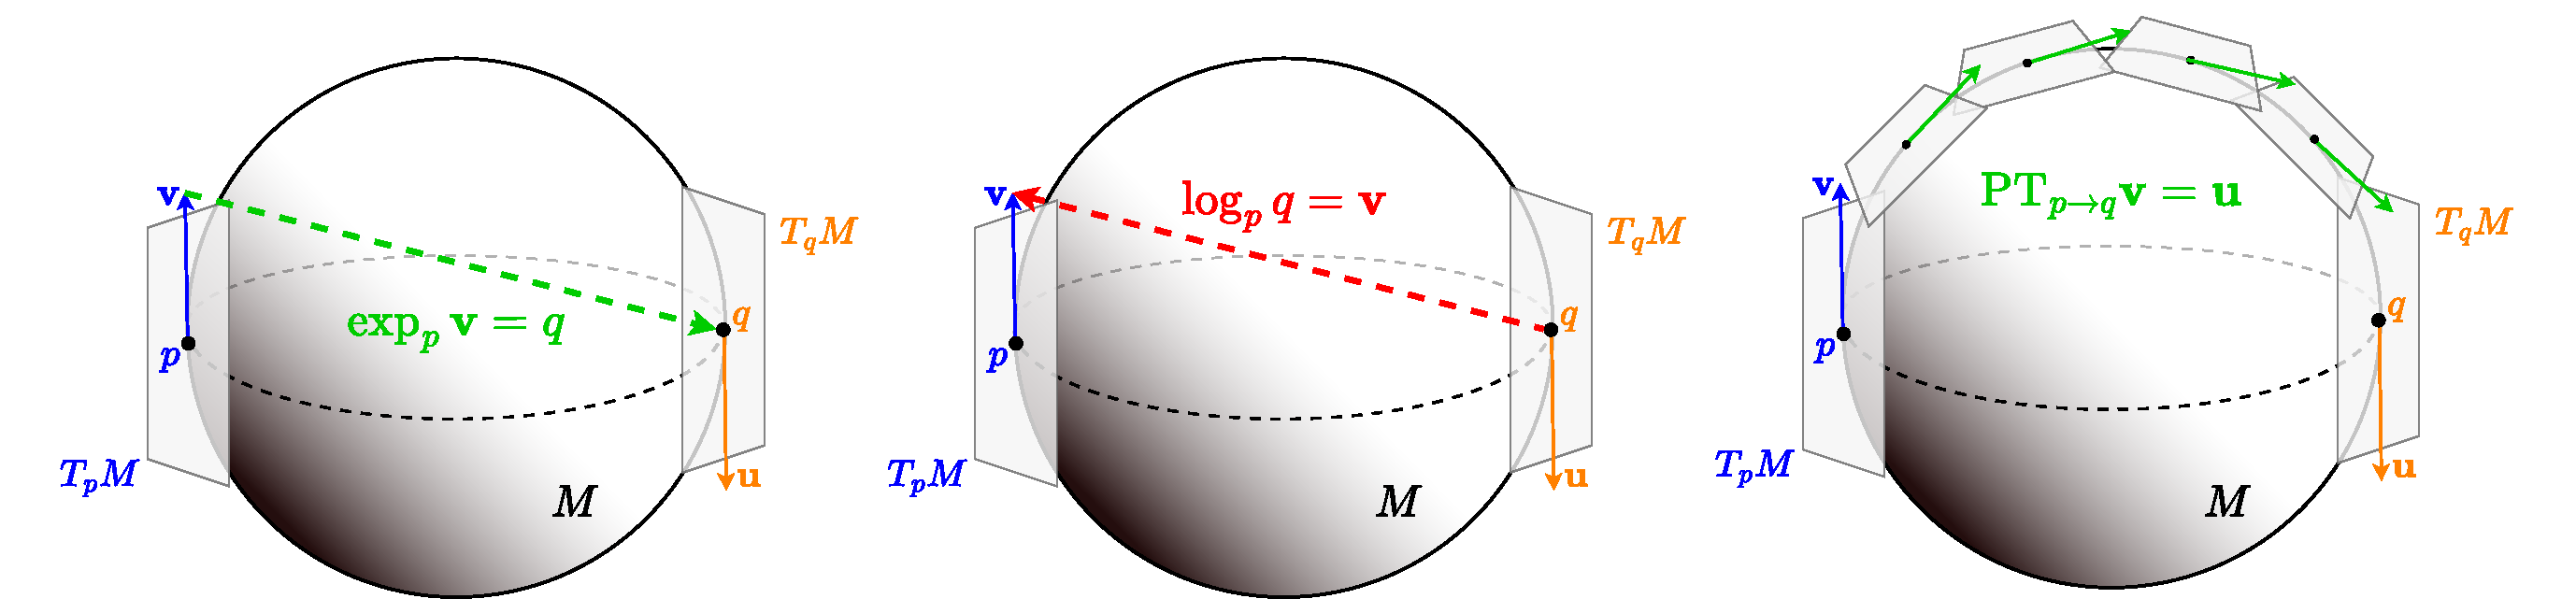
\includegraphics[width=\linewidth]{figures/manifolds.drawio.pdf}
    \caption{\label{fig:manifolds}\textbf{Visualizing the exponential, logarithmic, and parallel transport maps on a manifold.} The unique geodesic curve $\gamma$ between $p$ and $q$ with $\dot \gamma(0) = \mathbf{v}$ corresponds to the great circle of the sphere coinciding with the upper boundary in the diagrams.}    
\end{figure}

A smooth \textit{manifold} $M$ is a smooth topological space that is locally Euclidean. The local Euclidean structure is represented by \textit{charts} mapping open sets $U \subset M$ to $\R^n$. A set of charts covering the entire manifold is called an \textit{atlas}, and smoothness arises from the transitions between overlapping charts being smooth functions. Each point $x \in M$ is equipped with a tangent space $T_x M$ that is a vector space containing vectors tangent to $M$, such as velocities. In addition to being a smooth manifold, a Riemannian manifold also contains a Riemannian metric $g$ that defines an inner product $\langle u, v \rangle_g = u^T G v$ for $u, v \in T_x M$ and positive definite matrix $G$. A metric most importantly enables us to define angles and distances over the manifold as $\Vert u \Vert_g = \sqrt{\langle u, u\rangle_g} = \sqrt{u^T G u}$ and $\cos \theta = \frac{\langle u, v \rangle_g}{\Vert u \Vert_g \Vert v \Vert_g}$. 

A \textit{curve} is a smooth function $\gamma: [0, 1] \to M$, and tangent vectors $v \in T_x M$ can be expressed as time derivatives $\dot \gamma(t)$ of curves with $\gamma(t) = x$. Using the metric $g$, we can measure the length of a curve by computing the length of the tangent vector at each point along the curve:
\begin{equation}
    \vert \gamma \vert =
    \int_0^1 \Vert \dot \gamma (t) \Vert_g^2 dt.
\end{equation}
The ``shortest'' curve in this sense connecting two points $x,y\in M$ is called a \textit{geodesic}. We can thus define a distance between two points as the length of a (not necessarily unique) geodesic connecting them. 

A manifold is also equipped with three operations that we will make use of: the \textit{exponential map}, the \textit{logarithmic} map, and \textit{parallel transport} (see Figure \ref{fig:manifolds} for a visual depiction). The exponential map $\exp_x: T_x M \to M$ at a point $x \in M$ maps a tangent vector $v$ to the point $\gamma(1) \in M$ where $\gamma$ is the unique geodesic satisfying $\gamma(0) = x$ and $\dot \gamma(0) = v$. The logarithmic map $\log_x: M \to T_x M$ maps a point $y \in M$ back to the tangent vector $v := \dot \gamma (0)$. It is generally the inverse of the exponential map. Finally the parallel transport map $\text{PT}_{x \to y}: T_x M \to T_y M$ transports a tangent vector $v := \dot \gamma(0)$ along the geodesic with $\gamma(1) = y$ keeping the lengths and angles between the transported vectors constant. Together, these three operations allow us to move along geodesics with tangent vectors as the velocities, and transport tangent vectors to the same tangent space to be able to compute distances between them, which are all steps required to build a flow model over a Riemannian manifold. 

\subsection{Flow Models over Manifolds}

Riemannian flow matching (RFM) \citep{chenRiemannianFlowMatching2023} extends the flow matching framework to Riemannian manifolds. As the three key design choices, we need to define a coupling $q$, conditional probability paths $p_t$, and a conditional vector field $u_t$. 

A coupling can be defined simply by sampling $x_0 \sim p_0$ and $x_1 \sim p_1$ independently, or with a mini-batch optimal transport map with the distances defined above using geodesics. For $t\in [0,1]$, the geodesic interpolation $x_t \sim p_t(x_t \mid x_0, x_1)$ (analogous to linear interpolation in Euclidean space) between $x_0$ and $x_1$ is computed as 
\begin{equation}
    x_t := \exp_{x_0}(t \log_{x_0} x_1)
\end{equation}
and the conditional vector field $u_t$ as
\begin{equation}
    u_t(x_t \mid x_0, x_1) := \frac{\log_{x_t}x_1}{1 - t}.
\end{equation}
Finally to solve the ODE, we compute one Euler integration step as
\begin{align}
    dx_t &= u_t(x_t)dt \\
    x_{t + 1} &= \exp_{x_t}(v_\theta(t, x_t) \Delta t)
\end{align}
where $\Delta t$ is the step size. 


\section{Computing Likelihoods} \label{section:computing_likelihoods}

In earlier normalizing flows that aim to learn a static mapping between the two distributions \citep{rezendeVariationalInferenceNormalizing2015}, given source samples $x_0 \sim p_0$, likelihoods of the generated samples $z = f(x_0) \approx p_1$  can be computed exactly via the change of variables formula
\begin{equation} \label{eq:static_cov}
    \log p_1(z) = \log p_0(z) - \log \det \left\vert J_f(z) \right\vert
\end{equation}
where $J_f$ is the Jacobian of $f$. Thus, we can obtain exact likelihoods for the generated samples by taking the determinant of the Jacobian of the normalizing flow. Since Jacobian computations can be costly, this has motivated work on designing normalizing flows with easier to compute Jacobians, such as RealNVP \citep{dinhDensityEstimationUsing2017}. 

% Note that the terminology/notation etc are already set here
In a \textit{continuous normalizing flow} on the other hand, the \textit{instantaneous change of variables} formula \citep{chenNeuralOrdinaryDifferential2018a} defines the change in probability mass through time. Given that the vector field $v_t$ is continuous in $t$ and uniformly Lipschitz continuous in $\R^d$, it holds that
\begin{align} \label{eq:continuous_cov}
    \frac{d \log p_t(\phi_t(x))}{dt} &= - \divergence(v_t(\phi_t(x))) \\
                                     &= - \trace \left( \frac{d v_t(\phi_t(x))}{dt} \right)
\end{align}
where $\frac{d v_t(\phi_t(x))}{dt} =: J_v(\phi_t(x))$ is the Jacobian of the vector field. We integrate over time to compute the full change in probability:
\begin{equation} \label{eq:full_continuous_cov}
    \log p_1(\phi_1(x)) = \log p_0(\phi_0(x)) - \int_0^1 \trace(J_v(\phi_t(x))) dt.
\end{equation}
Then we can integrate the Jacobian trace of the vector field through time (simultaneously with sampling) to obtain exact likelihoods for the generated samples. 

\subsection{Faster Likelihoods Through Trace Estimation} \label{section:trace_estimation}

However, materializing the full Jacobian of the vector field can be prohibitively expensive, especially if the task is very high dimensional (as in our case) since the log determinant computation has a time complexity of $O(d^3)$ \citep{grathwohlFFJORDFreeformContinuous2018} without any restrictions on the structure of the Jacobian. 

To alleviate this problem, \citep{grathwohlFFJORDFreeformContinuous2018} propose to use the \textit{Hutchinson trace estimator} \citep{hutchinsonStochasticEstimatorTrace1990} for an unbiased estimate of the Jacobian trace of a square matrix: 
\begin{equation} \label{eq:hutchinson}
    \trace(J_v) = \bbE_{p(\epsilon)} \left[ \epsilon^T J_v \epsilon \right]
\end{equation}
where $p(\epsilon)$ is chosen such that $\bbE[\epsilon] = 0$ and $\Cov(\epsilon) = I$, typically a Gaussian or a Rademacher distribution. Then, we can use this estimator in place of the explicit trace computation in Equation \ref{eq:full_continuous_cov} and compute the likelihoods as
\begin{equation}
    \log p_1(\phi_1(x)) = \log p_0(\phi_0(x)) - \int_0^1 \bbE_{p(\epsilon)} \left[ \epsilon^T J_v(\phi_t(x)) \epsilon \right] dt.
\end{equation}

The performance benefit of using the Hutchinson trace estimator results from the fact that the Jacobian-vector product $J_v \epsilon$ can be computed very efficiently by automatic differentiation \citep{baydinAutomaticDifferentiationMachine2018}, giving the whole approach a time complexity of $O(d)$ only. Due to this significant performance improvement and being an unbiased estimate, the Hutchinson trace estimator has been widely used in the diffusion/flow model literature \citep{lipmanFlowMatchingGenerative2023,songScoreBasedGenerativeModeling2021a}.




% !TeX root = ../main.tex
% Add the above to each chapter to make compiling the PDF easier in some editors.

\chapter{Symmetries of Neural Network Weights}\label{section:geometry_of_nns}

Symmetries in data, such as rotation symmetries in molecules or translation symmetries in images, can be used to obtain useful inductive biases for ML models \citep{bronsteinGeometricDeepLearning2021,weilerEquivariantCoordinateIndependent2023}. By restricting the search space to functions that respect those symmetries, such inductive biases make training more data-efficient \citep{brehmerDoesEquivarianceMatter2024}. Since our data modality is neural network weights, taking the symmetries of neural networks into account can likewise make learning in weight space more effective. 

\begin{figure}[t!]
    \missingfigure[figwidth=\linewidth, figheight=6cm]{Diagram with permutation and scaling symmetries.}
    \caption{\label{fig:nn_sym} Symmetries of neural networks.}    
\end{figure}

Given a neural network $f$ with parameters $\theta$, we define a \textit{symmetry} as an operation $\phi$ that leaves the function computed by the neural network unchanged; i.e. $f_{\phi(\theta)}(x) = f_\theta(x)$. We are further interested only in the static symmetries that hold for any $\theta$ and thus can more reliably be used as inductive biases, rather than dynamic symmetries specific to a certain value of $\theta$. Such symmetries of neural network weights have been studied for a long time \citep{hecht-nielsenALGEBRAICSTRUCTUREFEEDFORWARD1990}, and are still key considerations for understanding the loss landscape and training dynamics of neural networks \citep{breaWeightspaceSymmetryDeep2019a,simsekGeometryLossLandscape2021,limEmpiricalImpactNeural2024,zhaoIMPROVINGCONVERGENCEGENERALIZATION2024}.

\section{Permutation and Scaling Symmetries of Neural Networks} \label{sec:perm_and_scale_sym}

A typical neural network with non-linear activations has two main kinds of symmetries: \textit{permutation symmetries} and \textit{scaling symmetries}. Permutation symmetries arise from the connectivity structure of the neural network, and scaling symmetries mainly arise from the particular non-linearities. 

More formally, consider a two-layer MLP with weight matrices $\W_1, \W_2$ and element-wise activations $\sigma$; i.e. $f_\theta(x) = \W_2 \sigma (\W_1x)$, ignoring the biases for simplicity but the following discussion applies to the biases as well. Let $\bP$ be an arbitrary permutation matrix. We can permute the hidden neurons, and apply the same permutation to their outgoing weights as well to keep the function unchanged:
\begin{equation}
    f_\theta(x) = \W_2 \sigma (\W_1x) = \W_2 \bP^T \sigma (\bP \W_1x).
\end{equation}
Since $\sigma$ is applied element-wise, we have $\W_2 \bP^T  \bP \sigma (\W_1x)$ which preserves the function as $\bP^T  \bP = \mathbf{I}$. Similarly, convolutional neural networks' channels can be permuted while preserving the function. More generally, \citet{limGraphMetanetworksProcessing2023} show that the permutation symmetries of any neural network correspond to graph automorphisms of its neural DAG, constructed with each edge corresponding to a parameter (e.g. directly the computational graph for MLPs, or with each filter corresponding to a node for CNNs).

In addition to these permutation symmetries, element-wise activation functions such as ReLU introduce further scaling symmetries to neural networks. For example, for the ReLU activation it holds for any real number $\lambda > 0$ that $\text{ReLU}(\lambda x) = \lambda \text{ReLU}(x)$. This means the input weights to a layer with ReLU activations can be multiplied with a positive number, and the function will remain unchanged as long as the output weights are scaled down with the same factor. Although we will mostly consider ReLU networks in the following sections, it is worth noting that such scaling symmetries exist for activation functions besides ReLU as well. \citep{godfreySymmetriesDeepLearning2022} have shown that symmetries resulting from activation functions can be associated with different \textit{intertwiner groups}, and provide concrete examples of these groups for various activation functions. 

\section{Linear Mode Connectivity}

\begin{figure}[t!]
    \missingfigure[figwidth=\linewidth, figheight=6cm]{Figure for mode connectivity.}
    \caption{\label{fig:mode_conn} Mode connectivity.}    
\end{figure}


Closely related to the literature on symmetries of neural network weights is the topic of \textit{linear mode connectivity}, concerned with finding (linear) low-loss paths between SGD-optimized weights. Finding such paths is useful for many downstream applications, such as ensembling neural networks \citep{garipovLossSurfacesMode2018a} by finding accurate weights with different representations without training, or model merging \citep{stoicaZipItMergingModels2024}.

\citet{garipovLossSurfacesMode2018a} first formulated the problem as finding parametrized curves between NN weights, minimizing the loss across the curve. It was later conjectured by \citet{entezariRolePermutationInvariance2022} that up to permutation symmetries, such low-loss paths are linear. The linear mode connectivity hypothesis has since then given rise to a fruitful research area \citep{ferbachProvingLinearMode2024,rossiPermutationSymmetriesBayesian2023,zhaoUnderstandingModeConnectivity2023}. 

For our purposes, modes being linearly connected would imply that finding the optimal permutations could effectively reduce the number of modes in the weight-space posterior, making it easier to approximate. Accounting for this multi-modality has been shown to improve the effectiveness of Bayesian neural networks \citep{sommerConnectingDotsModeConnectedness2024}. With this motivation, we next focus on the literature around finding such permutations. 

\section{Aligning Neural Networks}

The problem of finding a permutation of one neural network weights to obtain a linear low-loss path with another neural network, we call \textit{aligning} neural networks, has given rise to a high number of methods over years, the entirety of which could be a thesis in itself. For instance, \citep{ainsworthGitReBasinMerging2023} propose various approaches. The first is a data-based approach that matches the activations of models $A$ and $B$ of each layer,
\begin{equation}
    \bP^* = \arg\min_{\bP \in S_d} \sum_{i=1}^n \Vert \mathbf{Z}_A - \bP \mathbf{Z}_B \Vert ^2
\end{equation}
with $d$ dimensional activations $\mathbf{Z}$ for $n$ data points. This is an instance of the \textit{linear assignment problem} which can be solved in polynomial time \citep{crouseImplementing2DRectangular2016}. An alternative is to align the weights of the neural networks directly, which can again be reduced to a linear assignment problem and is more efficient since it requires no forward passes over the model, but sacrifices accuracy by ignoring the data. 

\citet{penaReBasinImplicitSinkhorn2023} propose a more flexible framework, making it possible optimize for any differentiable objective, and we also use their approach in the rest of our work. \citet{penaReBasinImplicitSinkhorn2023} start by relaxing the constraint of binary permutation matrix $\bP \in \Pi$ to obtain unconstrained $\mathbf{X} \in \R^{m\times n}$. Such a matrix can then be mapped to the space of binary permutation matrices via the \textit{Sinkhorn operator}:
\begin{equation} \label{eq:sinkhorn}
    S_\tau(\mathbf{X}) = \arg\max_{\bP \in \Pi} \langle \bP, \mathbf{X} \rangle_F + \tau h(\bP)
\end{equation}
where $F$ denotes the Frobenius norm and entropy $h(\bP) = - \sum \bP \log \bP$. Then the optimization is performed over $\R^{m \times n}$, and a binary permutation matrix is obtained through the Sinkhorn operator. 

The main advantage of the approach of \citet{penaReBasinImplicitSinkhorn2023} is that it can be used with arbitrary differentiable objectives. To align the parameters $\theta_A$ and $\theta_B$, with $\pi_\bP$ denoting the permutation applied to the weights, \citet{penaReBasinImplicitSinkhorn2023} propose three objectives. First is a straightforward weight-matching similar to \citep{ainsworthGitReBasinMerging2023}
\begin{equation}
    \mathcal{L}_{L2} := \Vert \theta_A - \pi_\bP (\theta_B) \Vert^2,
\end{equation}
followed by two data-based objectives. Minimizing the mid-point loss between the two weights as
\begin{equation}
    \mathcal{L}_{\text{Mid}} := \mathcal{L} \left( \frac{\theta_A + \pi_\bP (\theta_B)}{2} \right) 
\end{equation}
or the loss at a random intermediate point 
\begin{equation}
    \mathcal{L}_{\text{Rnd}} := \mathcal{L} \left( (1-\lambda)\theta_A + \lambda \pi_\bP (\theta_B) \right) 
\end{equation}
with $\lambda \sim \mathcal{U}(0,1)$. At the end, particularly the data-based losses result in more effective permutations than the method of \citep{ainsworthGitReBasinMerging2023}, and we choose to use the approach of \citet{penaReBasinImplicitSinkhorn2023} in the rest of our work also considering its flexibility. 

\section{Canonical Representations of Neural Networks}

This discussion around permutation and scaling symmetries of neural networks culminates with \textit{canonical representations} of neural networks, i.e. unique representations for each set of permutation/scale-symmetric neural networks, limiting our discussion to ReLU networks for simplicity. Following the work of \citep{pittorinoDeepNetworksToroids2022}, this can achieved in two steps given a set of neural networks $\{ \theta_i\}_i^N$:
\begin{enumerate}
    \item Align all neural networks to a single \textit{reference} neural network $\theta'$, using the approach of \citep{penaReBasinImplicitSinkhorn2023}. 
    \item For each intermediate layer $l$ and neuron $k$, scale down the incoming weights and biases by the norm of the incoming weight vector, $\vert w_k^l \vert^{-1}$, and the outgoing weights by $\vert w_k^l \vert$. Additionally for classification tasks, normalize the last layer's weights to $\sqrt{C}$, with $C$ the number of classes. This does not change the predicted label due to the argmax operation at the last layer. 
\end{enumerate}
With these two operations, the permutation and scaling symmetries are ``broken,'' as all the neural networks that compute the same function up to permutation and scaling are now mapped to the same point in weight space. Nevertheless, while the scaling symmetry is broken exactly, the permutation symmetry is broken up to an approximation since the alignment methods \citep{ainsworthGitReBasinMerging2023,penaReBasinImplicitSinkhorn2023} only output approximate solutions. For this reason, as we will describe in the next section, we use graph neural networks to fully account for the permutation symmetries. This canonicalization also gives a specific geometric structure to the set of neural network weights. Each neuron, characterized by its incoming weights, now lies on the unit hypersphere, and each layer in turn has a product geometry of hyperspheres. This enables the computation of geodesic paths and distances between neural networks. 

% !TeX root = ../main.tex
% Add the above to each chapter to make compiling the PDF easier in some editors.

\chapter{Graph Neural Networks \& MetaNets}\label{section:gnns}

% !TeX root = ../main.tex
% Add the above to each chapter to make compiling the PDF easier in some editors.

\section{Generative Models in Weight-Space}\label{section:gen_weight_models}

% !TeX root = ../main.tex
% Add the above to each chapter to make compiling the PDF easier in some editors.

\chapter{Method \& Design Choices}\label{chapter:method}

% !TeX root = ../main.tex
% Add the above to each chapter to make compiling the PDF easier in some editors.

\chapter{Experimental Results}\label{chapter:results}

{\color{red} SOME INTRO SUMMARIZING THE FINDINGS IN BULLET POINTS}

We describe the complete experimental setups in Appendix \ref{appendix:experimental_setups}.

\section{Euclidean Flow Between Two Gaussians} \label{sec:gaussian_flow}

\begin{figure}[h!]
    \centering
    \begin{subfigure}{0.47\linewidth}
        \centering
        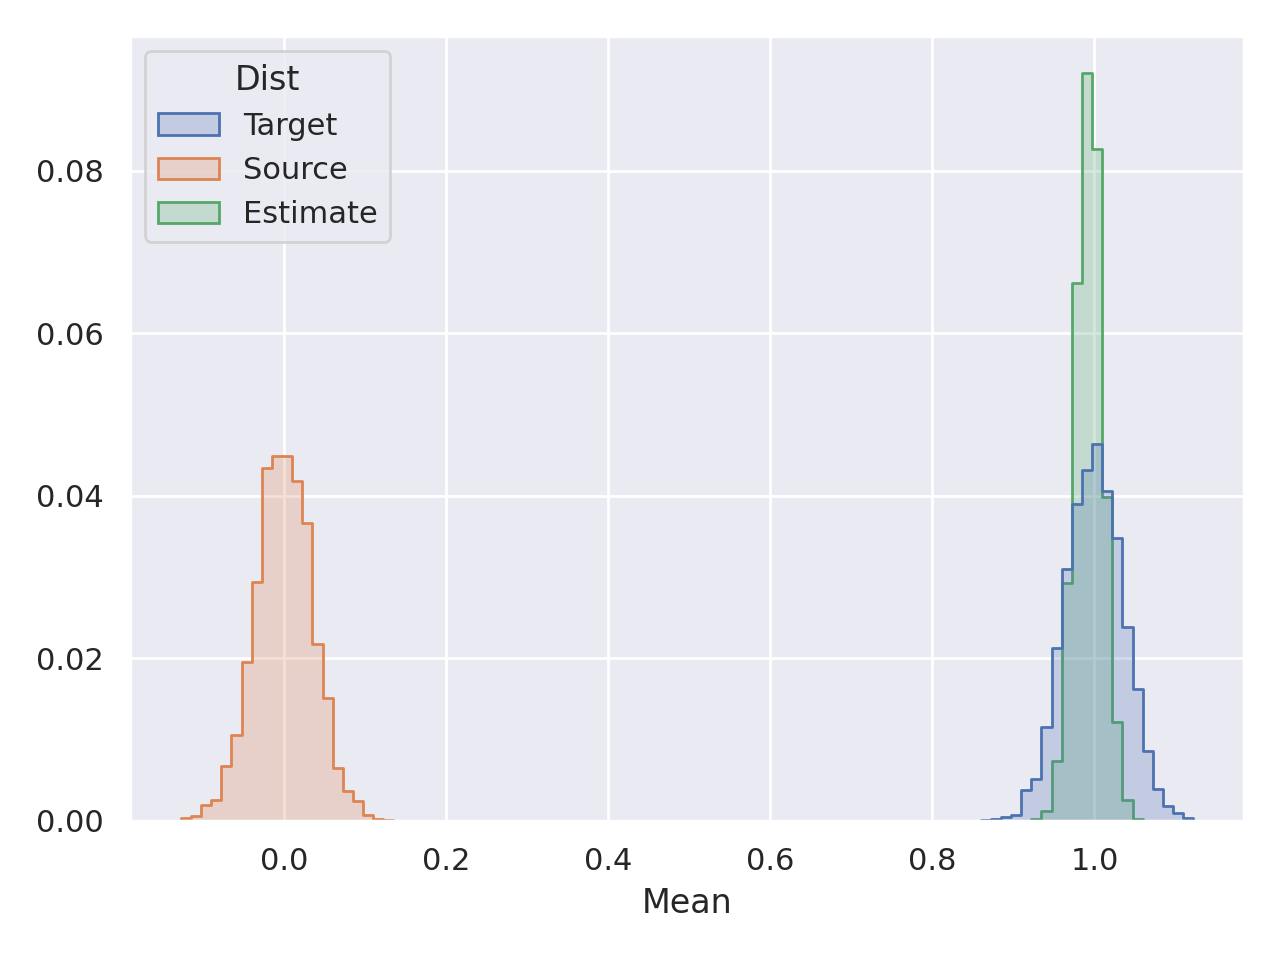
\includegraphics[width=\linewidth]{figures/gaussian/0.png}
        \caption{Deterministic sampling $(\varepsilon = 0)$}
        \label{fig:gaussian_deterministic}
    \end{subfigure}
    \begin{subfigure}{0.47\linewidth}
        \centering
        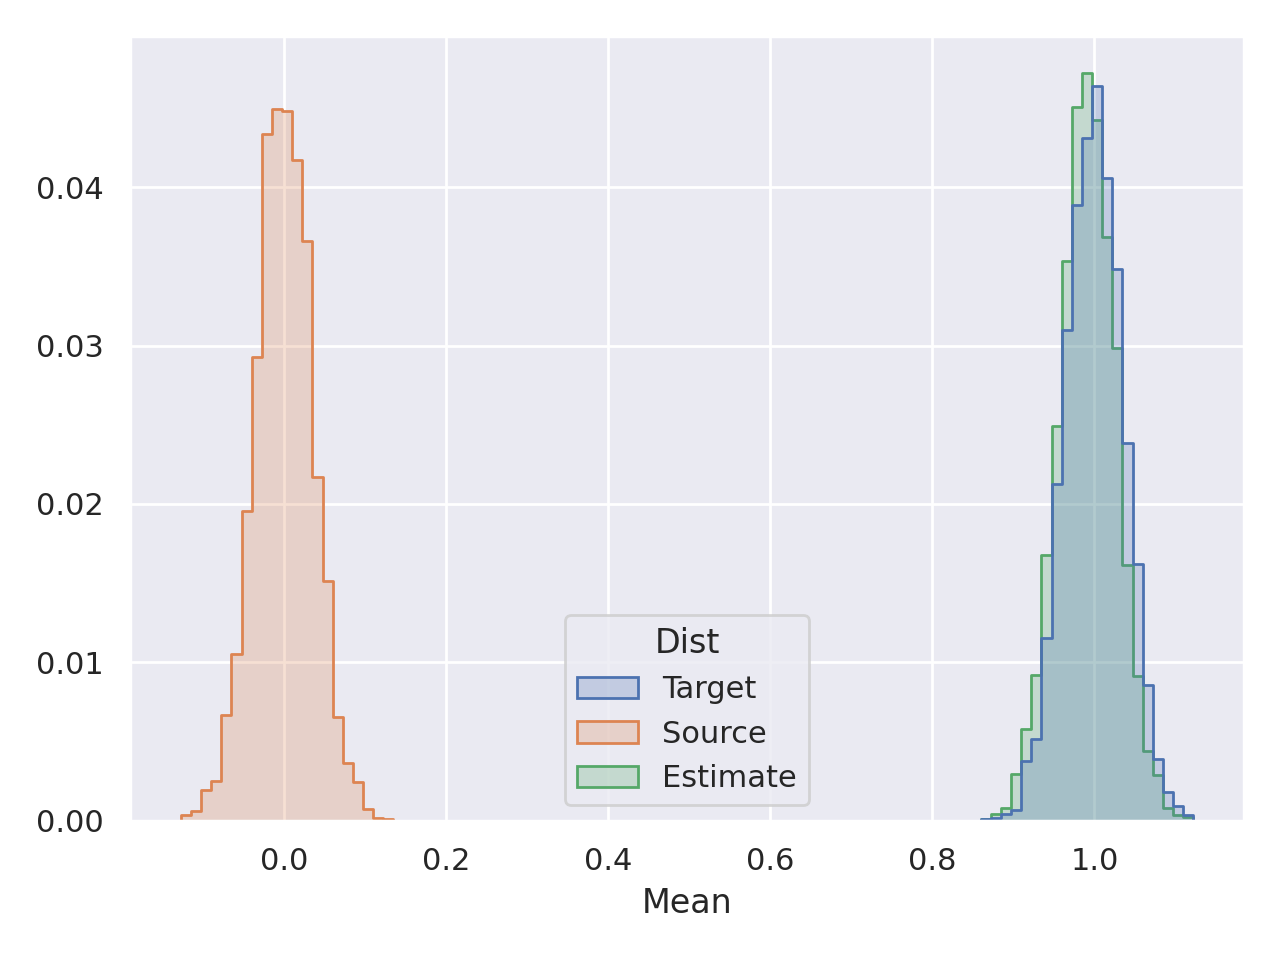
\includegraphics[width=\linewidth]{figures/gaussian/0.05.png}
        \caption{Stochastic sampling $(\varepsilon = 0.05)$}
        \label{fig:gaussian_stochastic}
    \end{subfigure}
    \caption{\label{fig:gaussian-results}\textbf{Histograms for the means of the weights generated by a Euclidean flow trained between two Gaussian distributions.} The flow fails to capture the variance in the target distribution with deterministic sampling, but this is corrected by stochastic sampling with $\varepsilon = 0.05$.} 
\end{figure}

To verify our approach of learning a flow model in weight-space, we begin our evaluation the toy task of learning a flow between two Gaussian distributions. The neural network is a small MLP with 30 input, two output dimensions, and two hidden layers of 16 neurons. We sample $X_0 \sim p_0 := \N(0, \mathbf{I})$ and $X_1 \sim p_1 := \N(1, \mathbf{I})$, and train our Euclidean flow to map $p_0$ to $p_1$ with independent coupling $q(x_0, x_1) = p_0(x_0)p_1(x_1)$. This is a relatively simpler task than learning over actual weights since each weight is sampled independently. 

Figure \ref{fig:gaussian-results} shows histograms of the means of the weights sampled from the flow with 100 Euler steps, and either deterministic or stochastic $(\varepsilon=0.05)$ sampling. Independent of the sampling method used, the flow covers the high-density center of the target distribution well, but the weights sampled deterministically fail to capture the variance in the target distribution. Stochastic sampling however appears to correct for this over-saturation and leads to more diverse samples. Overall, these results validates the feasability of learning a flow model in weight-space using graph neural networks, and we move on to tasks involving actual learned weights. 


\section{Classification with a Small Model}

Describe the model as well, mention why we can go geometric since relu activations. 

\begin{table}[h!]
    \centering
    \begin{tabular}{lll}
        \toprule
        \textbf{Flow}  & \textbf{Accuracy} & \textbf{Loss} \\
        \midrule
        Euclidean  & 0.998 ± 0.006 & 0.101 ± 0.05 \\ 
        Euclidean (aligned)  & 0.998 ± 0.006 & 0.07 ± 0.04 \\
        \midrule
        Normalized  & 0.993 ± 0.009 & 0.027 ± 0.014 \\
        Normalized (aligned)  & 0.989 ± 0.011 & 0.03 ± 0.015 \\
        \midrule
        Geometric  & 0.815 ± 0.279 & 0.525 ± 0.81 \\
        Geometric (aligned)  & 0.819 ± 0.277 & 0.551 ± 0.872 \\
        \midrule
        \textbf{Target} & 0.992 ± 0.01 & 0.048 ± 0.032 \\
        \bottomrule
    \end{tabular}
    \caption{\label{tab:uci_class_table}UCI results direct sample quality}
\end{table}

\begin{figure}[h!]
    \centering
    \begin{subfigure}{0.47\linewidth}
        \centering
        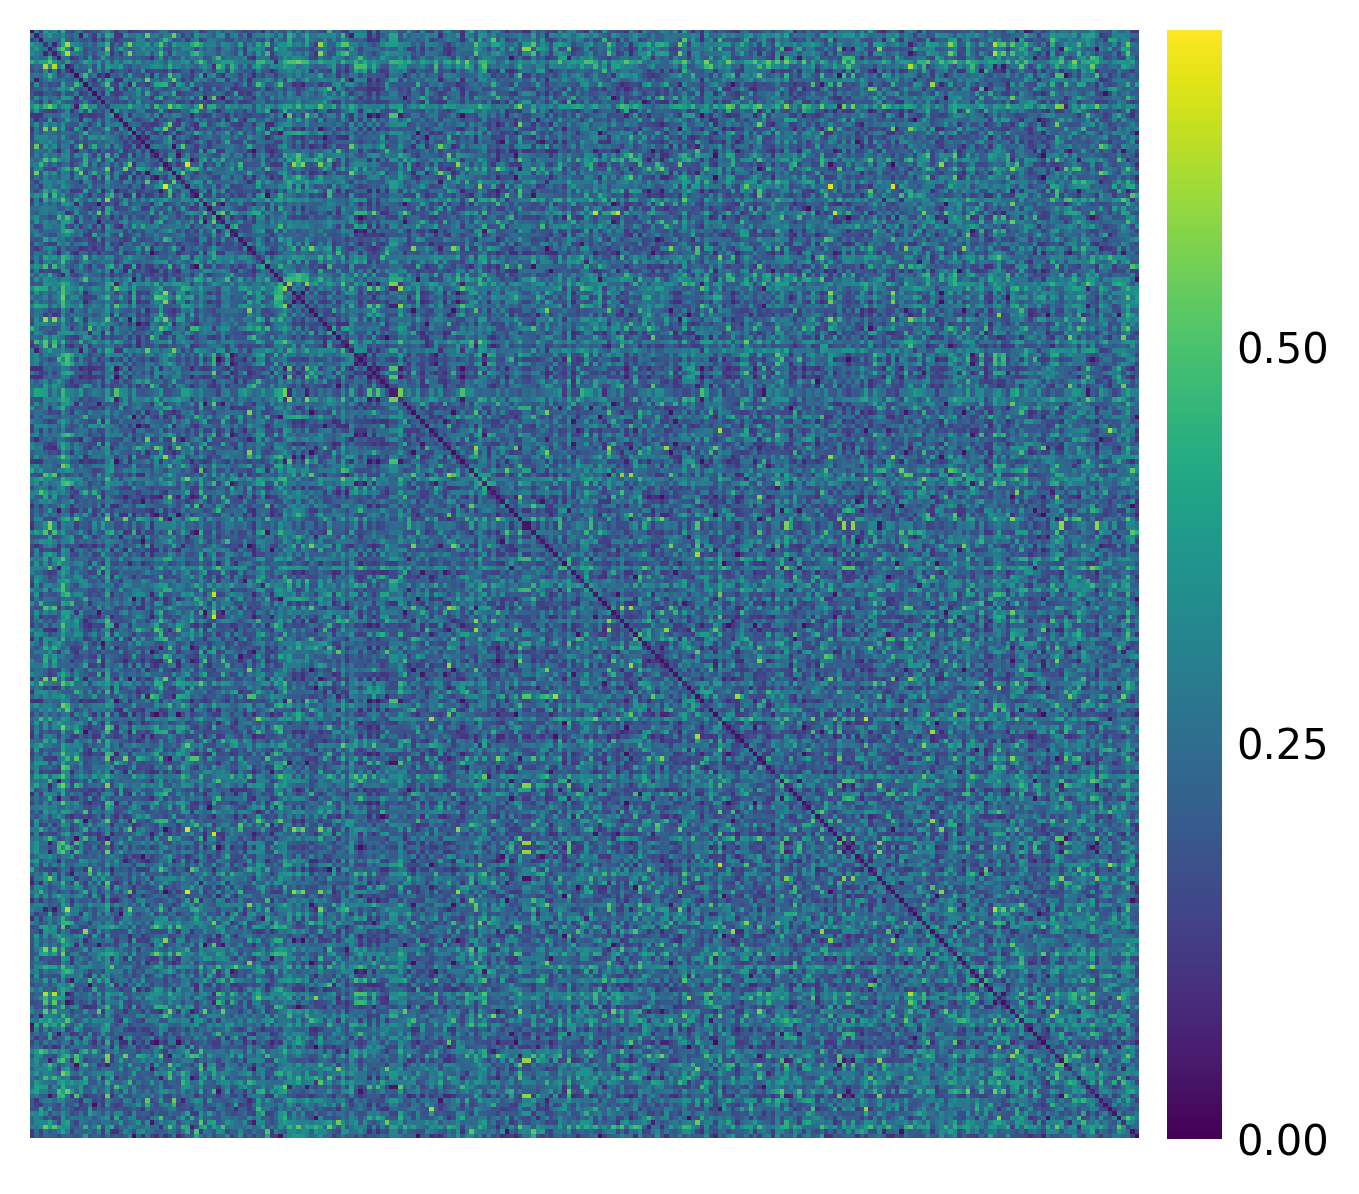
\includegraphics[width=\linewidth]{figures/uci_17/uci_17_unaligned.png}
        \caption{Unaligned (0.244 ± 0.009)}
        \label{fig:uci_unaligned}
    \end{subfigure}
    \begin{subfigure}{0.47\linewidth}
        \centering
        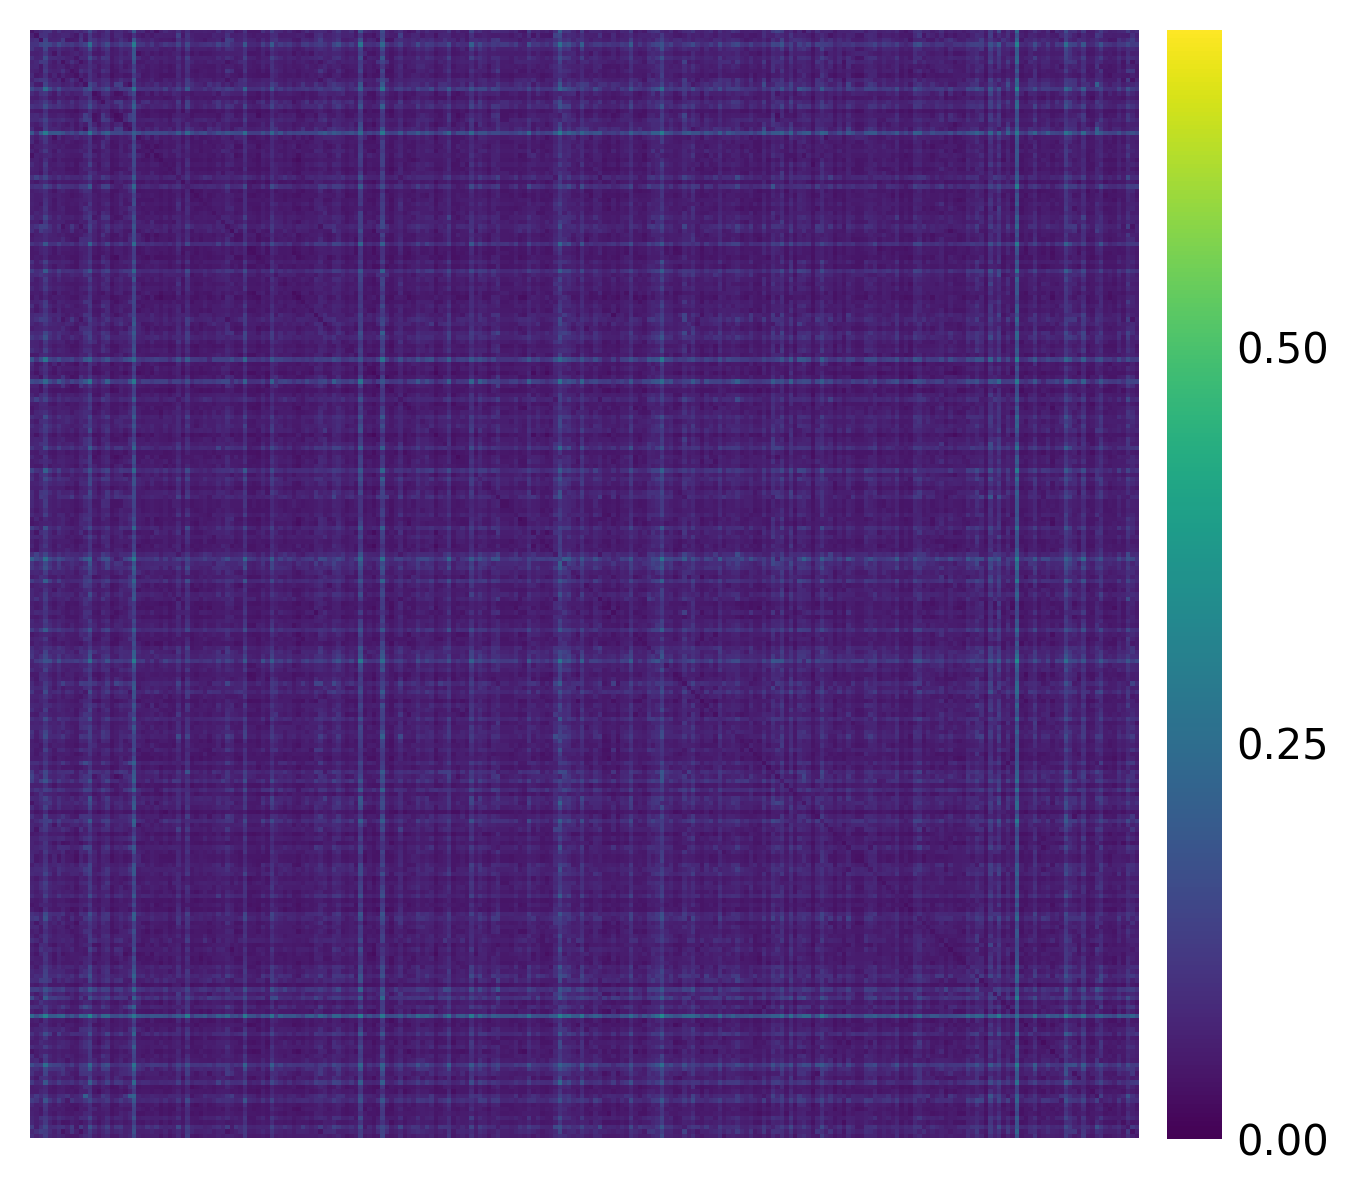
\includegraphics[width=\linewidth]{figures/uci_17/uci_17_aligned.png}
        \caption{Aligned (0.070 ± 0.001)}
        \label{fig:uci_aligned}
    \end{subfigure}
    \caption{\label{fig:uci_alignment}\textbf{Loss barriers for 250 weights across different optimization trajectories} (mean and standard deviations in parentheses). Aligning all weights to a single reference significantly reduces the loss barriers between the weights. } 
\end{figure}

\begin{figure}[h!]
    \centering
    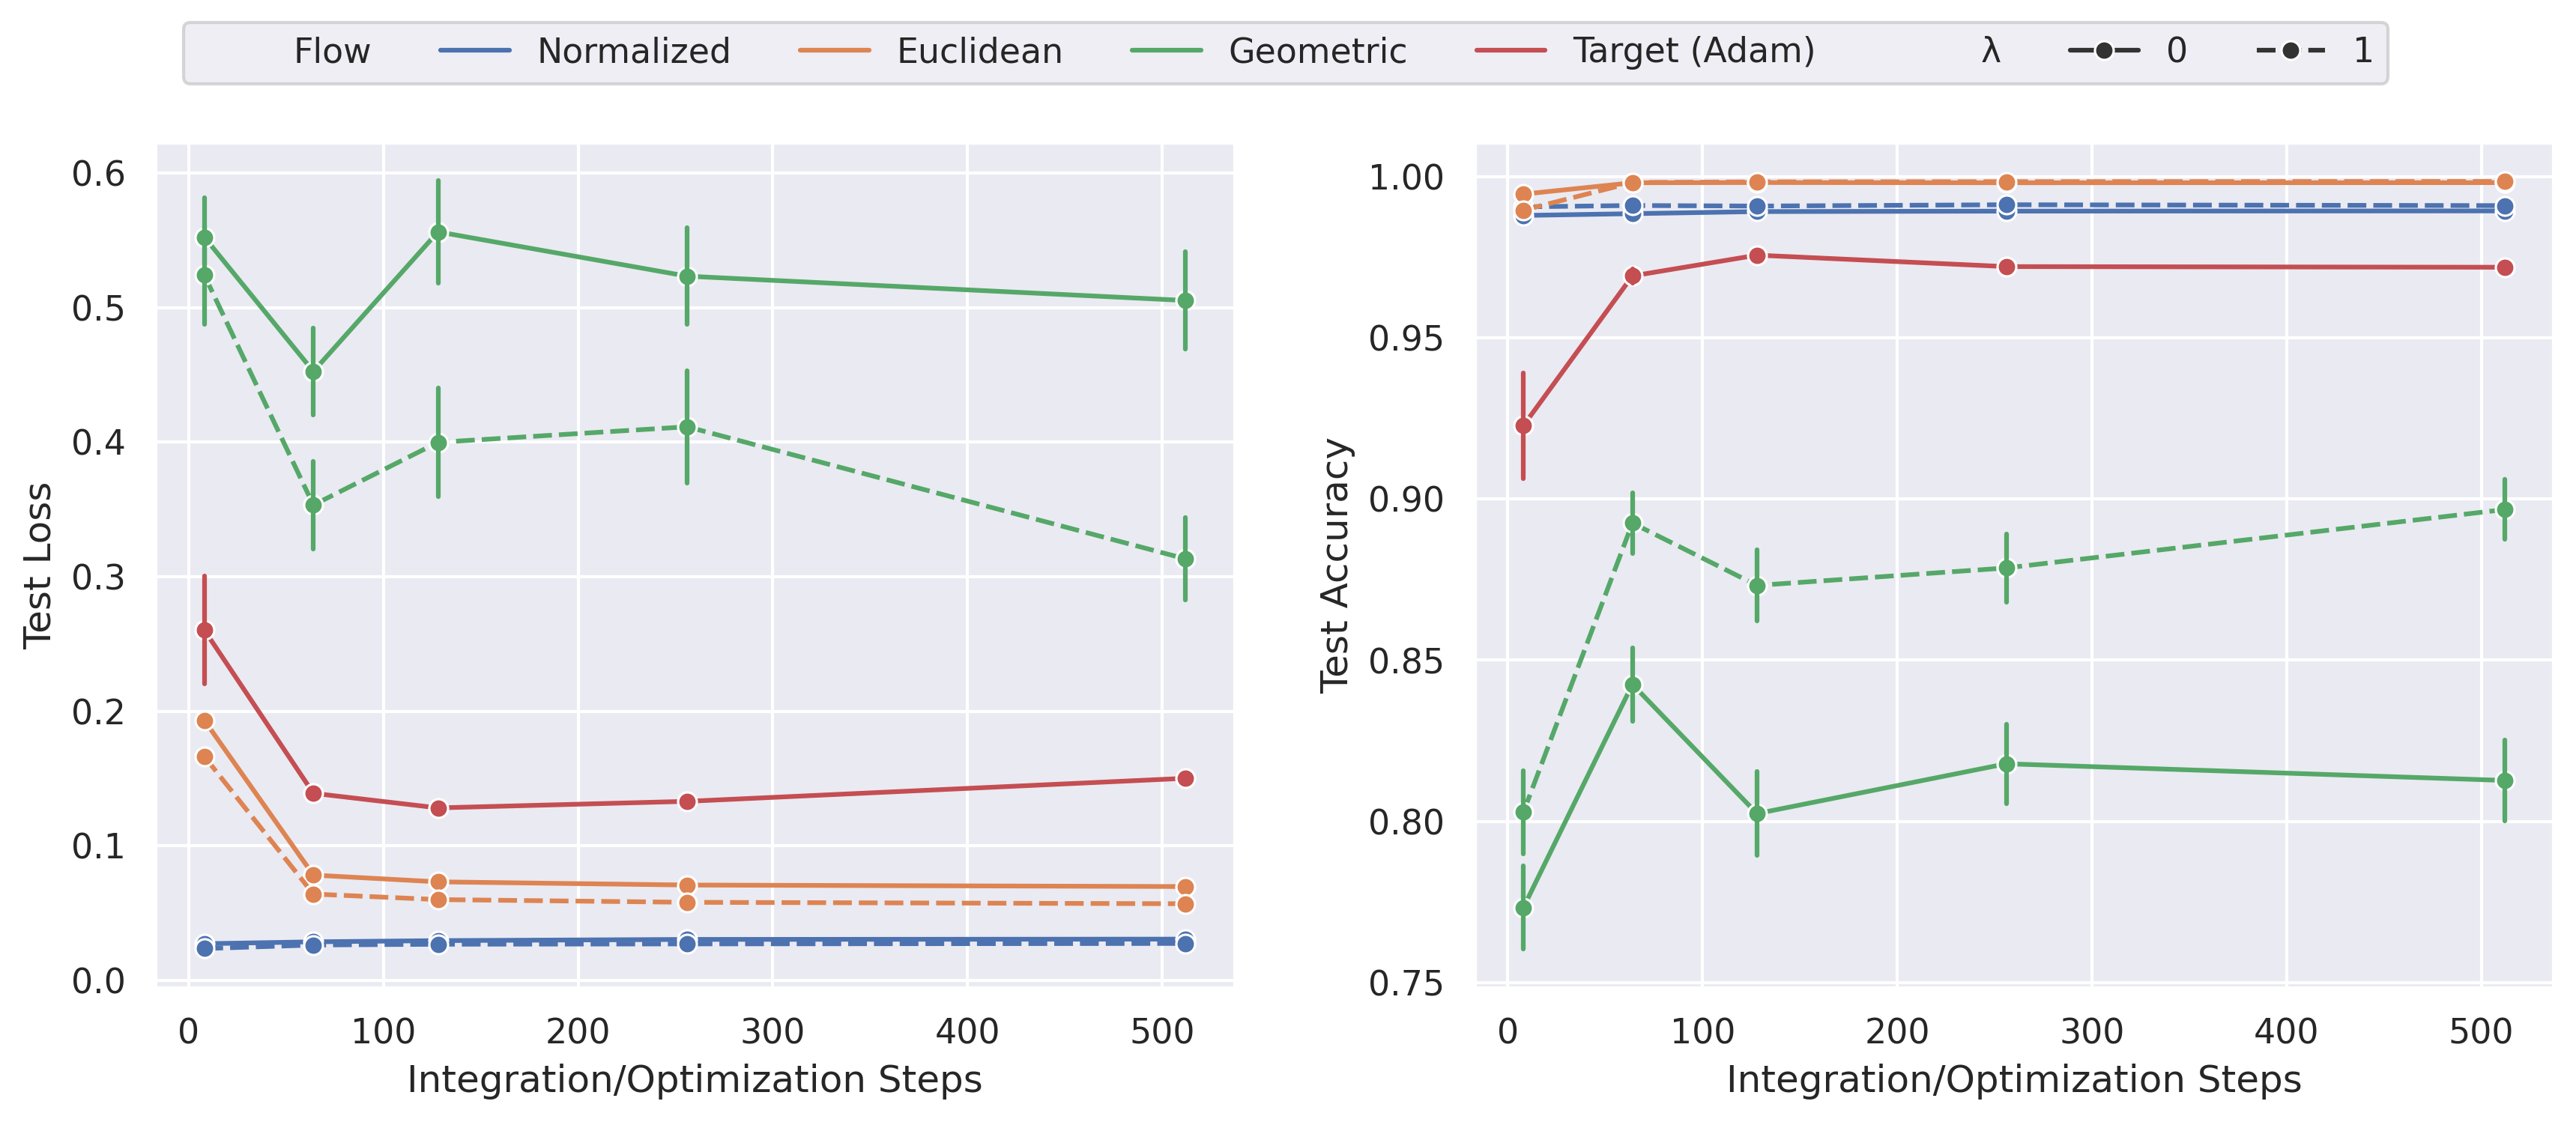
\includegraphics[width=\linewidth]{figures/uci_17/uci_17_steps_both.png}
    \caption{\label{fig:uci_steps}\textbf{Comparing the quality of the generated weights with Adam-optimized weights.} Weights generated by the Euclidean and Normalized flows have higher accuracy and lower loss than Adam-optimized weights, while the Geometric flow generated less accurate weights. Guidance during sampling improves sample quality.} 
\end{figure}




{\color{orange} how this task is easy since convex after alignment etc etc, but need to show with results}

% !TeX root = ../main.tex
% Add the above to each chapter to make compiling the PDF easier in some editors.

\chapter{Discussion}\label{chapter:discussion}

\section{Future Directions}

While we have demonstrated that generative models in weight-space trained via the flow matching objective can generate high-quality samples and that taking into account the geometry of the neural network weights can make such flows more effective, applying modern generative models to neural network weights is still an active problem with many fruitful potential future directions. {\color{cyan} I am not happy with this, maybe change after the rest is done.}

\subsection{More Fine-Grained Geometric Considerations}

Our flows so far are built for MLPs and only take into account the permutation symmetries between subsequent layers and scaling symmetries resulting from the use of ReLU activations. However, as outlined in previous work \citep{kofinasGraphNeuralNetworks2024,limGraphMetanetworksProcessing2023}, different architectural choices such as convolutions, residual connections, or transformer blocks induce different kinds of symmetries that can be captured by constructing the neural graphs accordingly. The same GNN architectures, such as the Relational Transformer we have used, can then be used for learning tasks over these graphs. 

Different activation functions also induce different symmetries \citep{godfreySymmetriesDeepLearning2022} which can be used to embed neural networks into different manifolds, similar to our embedding of ReLU MLPs on a product of hyperspheres following \citep{pittorinoDeepNetworksToroids2022}. Since generative modeling frameworks such as flow matching can readily be applied to different manifolds \citep{chenRiemannianFlowMatching2023}, including the use of data-dependent metrics \citep{kapusniakMetricFlowMatching2024}, extending our flow models to different kinds of symmetries represents another potentially valuable line of work. 

Another future direction related to symmetries in weight-space is to account for data-dependent symmetries \citep{zhaoSymmetriesFlatMinima2023} that arise from the data the model is trained on rather than the static symmetries in the previous paragraph that are valid for all instantiations of the same architecture. Recent work attempting to find these symmetries in an automated way \citep{zhaoFindingSymmetryNeural2024} can also be useful building blocks in this light. 

Finally, certain functional constraints in neural networks such as group equivariance are often imposed through constraints on the neural networks' weights \citep{weilerEquivariantCoordinateIndependent2023}. If the base model has such constraints, accounting for them while designing the flow as well could reduce the effective dimensionality of the problem considerably and lead to more effcient flows. 

\subsection{Generative Modeling and Training}

While each our flows is trained on a single architecture and dataset to push-forward a single source distribution to a single target distribution, a single flow that could potentially learn to map different source distributions (e.g. corresponding to the same base architecture on different datasets, or different architectures on the same dataset) could be a more directly useful tool. This would essentially correspond to a setting where the model learns to model a vector field not in weight-space, but in the space of probability distributions. Generalizations of the flow matching framework to this setting, such as Meta Flow Matching \citep{atanackovicMetaFlowMatching2024a} and Wasserstein Flow Matching \citep{havivWassersteinFlowMatching2024} could be useful building blocks for such a flow, as well as the publicly available model zoos \citep{schurholtModelZoosDataset2022}. This approach could lead to weight-space ``foundation models'' that are trained over a diverse set of tasks and can be adapted to specific use cases by fine-tuning on a single task. While this would be instance of meta-learning \citep{hospedalesMetaLearningNeuralNetworks2022}, it would be have the added benefit of obtaining a probability distribution over solutions rather than point estimates. 

Furthermore, the requirement of sample-based training can also be relaxed by utilizing recent work on generative modeling not necessarily requiring samples \citep{vargasTransportMeetsVariational2023,akhound-sadeghIteratedDenoisingEnergy2024}. In particular, iDEM \citep{akhound-sadeghIteratedDenoisingEnergy2024} learns a sampler with access to the energy function and its gradient (and optionally samples from the posterior) without having to simulate the forward and backward trajectories of the sampling process, making it potentially useful in high-dimensional spaces such as neural network weights. 

\subsection{Sampling and Guidance}

While we sample using an Euler ODE solver and perform guidance during sampling only using the base task gradients, the sampling phase has a richer design space that can be utilized to obtain faster and more controllable flows. To begin with, higher-order ODE solvers can be used to reduce the approximation error to the learned vector field at the cost of longer sampling times. Distillation methods such as Flow Map Matching \citep{boffiFlowMapMatching2024} and Consistency Flow Matching \citep{yangConsistencyFlowMatching2024} can be utilized to instead speed up the sampling process.  

Using a generative modeling framework such as flow matching also enables guidance methods beyond using task gradients. First, any differentiable objective can be used in place of the task loss to guide the sampling process. Performing classifier-free guidance is also possible for flow models \citep{zhengGuidedFlowsGenerative2023}, to instead condition the sampling process on a variable such as the desired loss, as also done in weight-space with diffusion models in \citet{peeblesLearningLearnGenerative2022}. Finally an alternative conditioning approach in flow matching is to differentiate through the ODE sampling process to optimize the initial point $x_0$ so that the solution $x_1$ minimizes a loss function \citep{ben-hamuDFlowDifferentiatingFlows2024}. This and future work for controllable sampling in flow models can be adapted to weight-space to condition flows on desired quantities or objectives such as adversarial robustness. 

\subsection{Use Cases}
\begin{itemize}
    \item implicit neural representations, but not learning
    \item 
\end{itemize}

% !TeX root = ../main.tex
% Add the above to each chapter to make compiling the PDF easier in some editors.

\chapter{Conclusion \& Future Work}\label{chapter:conclusion}

\appendix{}

% !TeX root = ../main.tex
% Add the above to each chapter to make compiling the PDF easier in some editors.

\chapter{Experimental Setups}\label{appendix:experimental_setups}

\section*{Implementation Details and Computational Resources}

Our flows were primarily implemented in PyTorch \citep{paszkePyTorchImperativeStyle2019a}, building on the weight-space GNN and graph construction implementation of \citep{kofinasGraphNeuralNetworks2024} and with our custom flow matching implementation utilizing parts of the \texttt{torchcfm} package of \citep{tongImprovingGeneralizingFlowbased2023}. We have implemented a custom Euler solver to integrate our ODEs and used the \texttt{geoopt} package \citep{kochurovGeooptRiemannianOptimization2020} for geometric operations.

Throughout the experiments, we train all our models using a combination of NVIDIA A100 an H100 GPUs, with each model being trained on a single GPU. The training times range from around 6 hours for the smaller Euclidean flows to approximately 40 hours for the larger Geometric flows, although our implementation was not fully optimized for efficiency. 

\section*{Flow Between Gaussians (Section \ref{sec:gaussian_flow})}

\subsection*{Data}

\begin{itemize}
    \item $p_0 = \N(0, \mathbf{I}), p_1 = \N(1, \mathbf{I})$. 
    \item The model is an MLP with dimensions 30 - 16 - 16 - 2 and ReLU activations. 
\end{itemize}

\subsection*{Flow Architecture}
\begin{itemize}
    \item Relational Transformer \citep{diaoRelationalAttentionGeneralizing2023,kofinasGraphNeuralNetworks2024} with 5 layers and $d_E = 32$, GeLU activations \citep{hendrycksGaussianErrorLinear2023a}, one attention head. 
\end{itemize}

\subsection*{Flow/Training}
\begin{itemize}
    \item Independent coupling, $t \sim \text{Beta}(1, 2)$, Gaussian probability path with $\sigma = 0.001$, $x_1$ prediction.
    \item Trained for 20,000 iterations with batch size 16, using the Adam optimizer with initial learning rate 0.001.
\end{itemize}

\section*{UCI Classification (Section \ref{sec:uci_classification})}

\subsection*{Data}

\begin{itemize}
    \item $p_0 = \N(0, 0.1 \mathbf{I})$. To obtain samples from $p_1$, we sample 100 models from $p_0$ and train each independently for 50 epochs with Adam. We ignore the first 10 epochs, and record one sample every four iterations after that. 
    \item We use the same MLP architecture as the Gaussian experiments. 
\end{itemize}

\subsection*{Flow Architecture}
\begin{itemize}
    \item Relational Transformer \citep{diaoRelationalAttentionGeneralizing2023,kofinasGraphNeuralNetworks2024} with 5 layers and $d_E = 64$, GeLU activations \citep{hendrycksGaussianErrorLinear2023a}, one attention head. 
\end{itemize}

\subsection*{Flow/Training}
\begin{itemize}
    \item $t \sim \text{Beta}(1, 2)$, Gaussian probability path with $\sigma = 0.0001$, $x_1$ prediction.
    \item Trained for 250,000 iterations with batch size 32, using the Adam optimizer with initial learning rate 0.001.
\end{itemize}


\section*{MNIST Classification (Section \ref{sec:mnist_classification})}

\subsection*{Data}

\begin{itemize}
    \item $p_0 = \N(0, 0.1 \mathbf{I})$. For the target samples, we independently train 50 models for 25 epochs using SGD with momentum 0.9, learning rate 0.1, and weight decay 0.00001. We collect one sample every 10 iterations, discarding the first 5 epochs. 
    \item The base model is an MLP with 784 input and 10 output dimensions, and one hidden layer of 10 units. 
\end{itemize}

\subsection*{Flow Architecture}
\begin{itemize}
    \item Relational Transformer \citep{diaoRelationalAttentionGeneralizing2023,kofinasGraphNeuralNetworks2024} with 5 layers and $d_E = 32$, GeLU activations \citep{hendrycksGaussianErrorLinear2023a}, one attention head. 
\end{itemize}

\subsection*{Flow/Training}
\begin{itemize}
    \item $t \sim \text{Beta}(1, 2)$, Gaussian probability path with $\sigma = 0.00001$, $x_1$ prediction.
    \item Trained for $100,000$ iterations with batch size 8. 
\end{itemize}




\microtypesetup{protrusion=false}

\addchap{Abbreviations}
\begin{acronym}
	\itemsep-.25\baselineskip
	\acro{TUM}[TUM]{Technical University of Munich}
	% TODO: add acronyms
\end{acronym}

\listoffigures{}
\listoftables{}
\microtypesetup{protrusion=true}
\printbibliography

\end{document}
